%% bare_jrnl.tex
%% V1.4
%% 2012/12/27
%% by Michael Shell
%% see http://www.michaelshell.org/
%% for current contact information.
%%
%% This is a skeleton file demonstrating the use of IEEEtran.cls
%% (requires IEEEtran.cls version 1.8 or later) with an IEEE journal paper.
%%
%% Support sites:
%% http://www.michaelshell.org/tex/ieeetran/
%% http://www.ctan.org/tex-archive/macros/latex/contrib/IEEEtran/
%% and
%% http://www.ieee.org/



% *** Authors should verify (and, if needed, correct) their LaTeX system  ***
% *** with the testflow diagnostic prior to trusting their LaTeX platform ***
% *** with production work. IEEE's font choices can trigger bugs that do  ***
% *** not appear when using other class files.                            ***
% The testflow support page is at:
% http://www.michaelshell.org/tex/testflow/


%%*************************************************************************
%% Legal Notice:
%% This code is offered as-is without any warranty either expressed or
%% implied; without even the implied warranty of MERCHANTABILITY or
%% FITNESS FOR A PARTICULAR PURPOSE! 
%% User assumes all risk.
%% In no event shall IEEE or any contributor to this code be liable for
%% any damages or losses, including, but not limited to, incidental,
%% consequential, or any other damages, resulting from the use or misuse
%% of any information contained here.
%%
%% All comments are the opinions of their respective authors and are not
%% necessarily endorsed by the IEEE.
%%
%% This work is distributed under the LaTeX Project Public License (LPPL)
%% ( http://www.latex-project.org/ ) version 1.3, and may be freely used,
%% distributed and modified. A copy of the LPPL, version 1.3, is included
%% in the base LaTeX documentation of all distributions of LaTeX released
%% 2003/12/01 or later.
%% Retain all contribution notices and credits.
%% ** Modified files should be clearly indicated as such, including  **
%% ** renaming them and changing author support contact information. **
%%
%% File list of work: IEEEtran.cls, IEEEtran_HOWTO.pdf, bare_adv.tex,
%%                    bare_conf.tex, bare_jrnl.tex, bare_jrnl_compsoc.tex,
%%                    bare_jrnl_transmag.tex
%%*************************************************************************

% Note that the a4paper option is mainly intended so that authors in
% countries using A4 can easily print to A4 and see how their papers will
% look in print - the typesetting of the document will not typically be
% affected with changes in paper size (but the bottom and side margins will).
% Use the testflow package mentioned above to verify correct handling of
% both paper sizes by the user's LaTeX system.
%
% Also note that the "draftcls" or "draftclsnofoot", not "draft", option
% should be used if it is desired that the figures are to be displayed in
% draft mode.
%
\documentclass[journal]{IEEEtran}
%
% If IEEEtran.cls has not been installed into the LaTeX system files,
% manually specify the path to it like:
% \documentclass[journal]{../sty/IEEEtran}





% Some very useful LaTeX packages include:
% (uncomment the ones you want to load)


% *** MISC UTILITY PACKAGES ***
%
%\usepackage{ifpdf}
% Heiko Oberdiek's ifpdf.sty is very useful if you need conditional
% compilation based on whether the output is pdf or dvi.
% usage:
% \ifpdf
%   % pdf code
% \else
%   % dvi code
% \fi
% The latest version of ifpdf.sty can be obtained from:
% http://www.ctan.org/tex-archive/macros/latex/contrib/oberdiek/
% Also, note that IEEEtran.cls V1.7 and later provides a builtin
% \ifCLASSINFOpdf conditional that works the same way.
% When switching from latex to pdflatex and vice-versa, the compiler may
% have to be run twice to clear warning/error messages.





\usepackage[latin1]{inputenc}
% *** CITATION PACKAGES ***
%
%\usepackage{cite}
% cite.sty was written by Donald Arseneau
% V1.6 and later of IEEEtran pre-defines the format of the cite.sty package
% \cite{} output to follow that of IEEE. Loading the cite package will
% result in citation numbers being automatically sorted and properly
% "compressed/ranged". e.g., [1], [9], [2], [7], [5], [6] without using
% cite.sty will become [1], [2], [5]--[7], [9] using cite.sty. cite.sty's
% \cite will automatically add leading space, if needed. Use cite.sty's
% noadjust option (cite.sty V3.8 and later) if you want to turn this off
% such as if a citation ever needs to be enclosed in parenthesis.
% cite.sty is already installed on most LaTeX systems. Be sure and use
% version 4.0 (2003-05-27) and later if using hyperref.sty. cite.sty does
% not currently provide for hyperlinked citations.
% The latest version can be obtained at:
% http://www.ctan.org/tex-archive/macros/latex/contrib/cite/
% The documentation is contained in the cite.sty file itself.

\usepackage{times}
\usepackage{graphicx,marvosym}
\usepackage{setspace}
\usepackage{subfigure}
\usepackage{amssymb}
\usepackage{changepage}
\usepackage{listings}
\usepackage{multirow}
\usepackage{color}
\usepackage{colordvi}
\usepackage{array}

% *** GRAPHICS RELATED PACKAGES ***
%
\ifCLASSINFOpdf
  %\usepackage[pdftex]{graphicx}
  % declare the path(s) where your graphic files are
  % \graphicspath{{../pdf/}{../jpeg/}}
  % and their extensions so you won't have to specify these with
  % every instance of \includegraphics
  % \DeclareGraphicsExtensions{.pdf,.jpeg,.png}
\else
  % or other class option (dvipsone, dvipdf, if not using dvips). graphicx
  % will default to the driver specified in the system graphics.cfg if no
  % driver is specified.
  % \usepackage[dvips]{graphicx}
  % declare the path(s) where your graphic files are
  % \graphicspath{{../eps/}}
  % and their extensions so you won't have to specify these with
  % every instance of \includegraphics
  % \DeclareGraphicsExtensions{.eps}
\fi
% graphicx was written by David Carlisle and Sebastian Rahtz. It is
% required if you want graphics, photos, etc. graphicx.sty is already
% installed on most LaTeX systems. The latest version and documentation
% can be obtained at: 
% http://www.ctan.org/tex-archive/macros/latex/required/graphics/
% Another good source of documentation is "Using Imported Graphics in
% LaTeX2e" by Keith Reckdahl which can be found at:
% http://www.ctan.org/tex-archive/info/epslatex/
%
% latex, and pdflatex in dvi mode, support graphics in encapsulated
% postscript (.eps) format. pdflatex in pdf mode supports graphics
% in .pdf, .jpeg, .png and .mps (metapost) formats. Users should ensure
% that all non-photo figures use a vector format (.eps, .pdf, .mps) and
% not a bitmapped formats (.jpeg, .png). IEEE frowns on bitmapped formats
% which can result in "jaggedy"/blurry rendering of lines and letters as
% well as large increases in file sizes.
%
% You can find documentation about the pdfTeX application at:
% http://www.tug.org/applications/pdftex





% *** MATH PACKAGES ***
%
\usepackage[cmex10]{amsmath}
% A popular package from the American Mathematical Society that provides
% many useful and powerful commands for dealing with mathematics. If using
% it, be sure to load this package with the cmex10 option to ensure that
% only type 1 fonts will utilized at all point sizes. Without this option,
% it is possible that some math symbols, particularly those within
% footnotes, will be rendered in bitmap form which will result in a
% document that can not be IEEE Xplore compliant!
%
% Also, note that the amsmath package sets \interdisplaylinepenalty to 10000
% thus preventing page breaks from occurring within multiline equations. Use:
%\interdisplaylinepenalty=2500
% after loading amsmath to restore such page breaks as IEEEtran.cls normally
% does. amsmath.sty is already installed on most LaTeX systems. The latest
% version and documentation can be obtained at:
% http://www.ctan.org/tex-archive/macros/latex/required/amslatex/math/





% *** SPECIALIZED LIST PACKAGES ***
%
%\usepackage{algorithmic}
% algorithmic.sty was written by Peter Williams and Rogerio Brito.
% This package provides an algorithmic environment fo describing algorithms.
% You can use the algorithmic environment in-text or within a figure
% environment to provide for a floating algorithm. Do NOT use the algorithm
% floating environment provided by algorithm.sty (by the same authors) or
% algorithm2e.sty (by Christophe Fiorio) as IEEE does not use dedicated
% algorithm float types and packages that provide these will not provide
% correct IEEE style captions. The latest version and documentation of
% algorithmic.sty can be obtained at:
% http://www.ctan.org/tex-archive/macros/latex/contrib/algorithms/
% There is also a support site at:
% http://algorithms.berlios.de/index.html
% Also of interest may be the (relatively newer and more customizable)
% algorithmicx.sty package by Szasz Janos:
% http://www.ctan.org/tex-archive/macros/latex/contrib/algorithmicx/




% *** ALIGNMENT PACKAGES ***
%
%\usepackage{array}
% Frank Mittelbach's and David Carlisle's array.sty patches and improves
% the standard LaTeX2e array and tabular environments to provide better
% appearance and additional user controls. As the default LaTeX2e table
% generation code is lacking to the point of almost being broken with
% respect to the quality of the end results, all users are strongly
% advised to use an enhanced (at the very least that provided by array.sty)
% set of table tools. array.sty is already installed on most systems. The
% latest version and documentation can be obtained at:
% http://www.ctan.org/tex-archive/macros/latex/required/tools/


% IEEEtran contains the IEEEeqnarray family of commands that can be used to
% generate multiline equations as well as matrices, tables, etc., of high
% quality.




% *** SUBFIGURE PACKAGES ***
%\ifCLASSOPTIONcompsoc
%  \usepackage[caption=false,font=normalsize,labelfont=sf,textfont=sf]{subfig}
%\else
%  \usepackage[caption=false,font=footnotesize]{subfig}
%\fi
% subfig.sty, written by Steven Douglas Cochran, is the modern replacement
% for subfigure.sty, the latter of which is no longer maintained and is
% incompatible with some LaTeX packages including fixltx2e. However,
% subfig.sty requires and automatically loads Axel Sommerfeldt's caption.sty
% which will override IEEEtran.cls' handling of captions and this will result
% in non-IEEE style figure/table captions. To prevent this problem, be sure
% and invoke subfig.sty's "caption=false" package option (available since
% subfig.sty version 1.3, 2005/06/28) as this is will preserve IEEEtran.cls
% handling of captions.
% Note that the Computer Society format requires a larger sans serif font
% than the serif footnote size font used in traditional IEEE formatting
% and thus the need to invoke different subfig.sty package options depending
% on whether compsoc mode has been enabled.
%
% The latest version and documentation of subfig.sty can be obtained at:
% http://www.ctan.org/tex-archive/macros/latex/contrib/subfig/




% *** FLOAT PACKAGES ***
%
%\usepackage{fixltx2e}
% fixltx2e, the successor to the earlier fix2col.sty, was written by
% Frank Mittelbach and David Carlisle. This package corrects a few problems
% in the LaTeX2e kernel, the most notable of which is that in current
% LaTeX2e releases, the ordering of single and double column floats is not
% guaranteed to be preserved. Thus, an unpatched LaTeX2e can allow a
% single column figure to be placed prior to an earlier double column
% figure. The latest version and documentation can be found at:
% http://www.ctan.org/tex-archive/macros/latex/base/


%\usepackage{stfloats}
% stfloats.sty was written by Sigitas Tolusis. This package gives LaTeX2e
% the ability to do double column floats at the bottom of the page as well
% as the top. (e.g., "\begin{figure*}[!b]" is not normally possible in
% LaTeX2e). It also provides a command:
%\fnbelowfloat
% to enable the placement of footnotes below bottom floats (the standard
% LaTeX2e kernel puts them above bottom floats). This is an invasive package
% which rewrites many portions of the LaTeX2e float routines. It may not work
% with other packages that modify the LaTeX2e float routines. The latest
% version and documentation can be obtained at:
% http://www.ctan.org/tex-archive/macros/latex/contrib/sttools/
% Do not use the stfloats baselinefloat ability as IEEE does not allow
% \baselineskip to stretch. Authors submitting work to the IEEE should note
% that IEEE rarely uses double column equations and that authors should try
% to avoid such use. Do not be tempted to use the cuted.sty or midfloat.sty
% packages (also by Sigitas Tolusis) as IEEE does not format its papers in
% such ways.
% Do not attempt to use stfloats with fixltx2e as they are incompatible.
% Instead, use Morten Hogholm'a dblfloatfix which combines the features
% of both fixltx2e and stfloats:
%
% \usepackage{dblfloatfix}
% The latest version can be found at:
% http://www.ctan.org/tex-archive/macros/latex/contrib/dblfloatfix/




%\ifCLASSOPTIONcaptionsoff
%  \usepackage[nomarkers]{endfloat}
% \let\MYoriglatexcaption\caption
% \renewcommand{\caption}[2][\relax]{\MYoriglatexcaption[#2]{#2}}
%\fi
% endfloat.sty was written by James Darrell McCauley, Jeff Goldberg and 
% Axel Sommerfeldt. This package may be useful when used in conjunction with 
% IEEEtran.cls'  captionsoff option. Some IEEE journals/societies require that
% submissions have lists of figures/tables at the end of the paper and that
% figures/tables without any captions are placed on a page by themselves at
% the end of the document. If needed, the draftcls IEEEtran class option or
% \CLASSINPUTbaselinestretch interface can be used to increase the line
% spacing as well. Be sure and use the nomarkers option of endfloat to
% prevent endfloat from "marking" where the figures would have been placed
% in the text. The two hack lines of code above are a slight modification of
% that suggested by in the endfloat docs (section 8.4.1) to ensure that
% the full captions always appear in the list of figures/tables - even if
% the user used the short optional argument of \caption[]{}.
% IEEE papers do not typically make use of \caption[]'s optional argument,
% so this should not be an issue. A similar trick can be used to disable
% captions of packages such as subfig.sty that lack options to turn off
% the subcaptions:
% For subfig.sty:
% \let\MYorigsubfloat\subfloat
% \renewcommand{\subfloat}[2][\relax]{\MYorigsubfloat[]{#2}}
% However, the above trick will not work if both optional arguments of
% the \subfloat command are used. Furthermore, there needs to be a
% description of each subfigure *somewhere* and endfloat does not add
% subfigure captions to its list of figures. Thus, the best approach is to
% avoid the use of subfigure captions (many IEEE journals avoid them anyway)
% and instead reference/explain all the subfigures within the main caption.
% The latest version of endfloat.sty and its documentation can obtained at:
% http://www.ctan.org/tex-archive/macros/latex/contrib/endfloat/
%
% The IEEEtran \ifCLASSOPTIONcaptionsoff conditional can also be used
% later in the document, say, to conditionally put the References on a 
% page by themselves.




% *** PDF, URL AND HYPERLINK PACKAGES ***
%
%\usepackage{url}
% url.sty was written by Donald Arseneau. It provides better support for
% handling and breaking URLs. url.sty is already installed on most LaTeX
% systems. The latest version and documentation can be obtained at:
% http://www.ctan.org/tex-archive/macros/latex/contrib/url/
% Basically, \url{my_url_here}.




% *** Do not adjust lengths that control margins, column widths, etc. ***
% *** Do not use packages that alter fonts (such as pslatex).         ***
% There should be no need to do such things with IEEEtran.cls V1.6 and later.
% (Unless specifically asked to do so by the journal or conference you plan
% to submit to, of course. )


% correct bad hyphenation here
\hyphenation{op-tical net-works semi-conduc-tor}


\begin{document}
%
% paper title
% can use linebreaks \\ within to get better formatting as desired
% Do not put math or special symbols in the title.
\title{Hardware Reconfiguration Scheme Based on the Digital TV Signal}
%
%
% author names and IEEE memberships
% note positions of commas and nonbreaking spaces ( ~ ) LaTeX will not break
% a structure at a ~ so this keeps an author's name from being broken across
% two lines.
% use \thanks{} to gain access to the first footnote area
% a separate \thanks must be used for each paragraph as LaTeX2e's \thanks
% was not built to handle multiple paragraphs
%

\author{Rodrigo~R.~de~Oliveira, Lucas~C.~Cordeiro, ~Eddie~B.~L.~Filho,
        and~Vicente~F.~de~Lucena~Jr.% <-this % stops a space
\thanks{Rodrigo R. de Oliveira is with Universidade Federal do Amazonas -- UFAM, Manaus, Amazonas, Brazil, 69077-000 e-mail: rodrigo@dcc.ufam.edu.br.}% <-this % stops a space
\thanks{Lucas C. Cordeiro is with Universidade Federal do Amazonas -- UFAM, Manaus, Amazonas, Brazil, 69077-000 e-mail: lucascordeiro@ufam.edu.br.}% <-this % stops a space
\thanks{Vicente F. de Lucena Jr. is with Universidade Federal do Amazonas -- UFAM, Manaus, Amazonas, Brazil, 69077-000 e-mail: vicente@ufam.edu.br.}% <-this % stops a space
\thanks{Eddie B. L. Filho is with Centro de Ci�ncia, Tecnologia e Inova��o do P�lo Industrial de Manaus -- CT-PIM, Manaus, Amazonas, Brazil, 69057-040 e-mail: eddie@ctpim.org.br.}% <-this % stops a space
\thanks{Manuscript received Mar. xx, 2005; revised Aug. xx, 2013.}}
% note the % following the last \IEEEmembership and also \thanks - 
% these prevent an unwanted space from occurring between the last author name
% and the end of the author line. i.e., if you had this:
% 
% \author{....lastname \thanks{...} \thanks{...} }
%                     ^------------^------------^----Do not want these spaces!
%
% a space would be appended to the last name and could cause every name on that
% line to be shifted left slightly. This is one of those "LaTeX things". For
% instance, "\textbf{A} \textbf{B}" will typeset as "A B" not "AB". To get
% "AB" then you have to do: "\textbf{A}\textbf{B}"
% \thanks is no different in this regard, so shield the last } of each \thanks
% that ends a line with a % and do not let a space in before the next \thanks.
% Spaces after \IEEEmembership other than the last one are OK (and needed) as
% you are supposed to have spaces between the names. For what it is worth,
% this is a minor point as most people would not even notice if the said evil
% space somehow managed to creep in.



% The paper headers
\markboth{IEEE TRANSACTIONS ON BROADCASTING,~Vol.~xx, No.~x, July~2014}%
{Oliveira, Cordeiro, Filho and Lucena: Hardware Reconfiguration Scheme Based on the Digital TV Signal}
% The only time the second header will appear is for the odd numbered pages
% after the title page when using the twoside option.
% 
% *** Note that you probably will NOT want to include the author's ***
% *** name in the headers of peer review papers.                   ***
% You can use \ifCLASSOPTIONpeerreview for conditional compilation here if
% you desire.




% If you want to put a publisher's ID mark on the page you can do it like
% this:
%\IEEEpubid{0000--0000/00\$00.00~\copyright~2012 IEEE}
% Remember, if you use this you must call \IEEEpubidadjcol in the second
% column for its text to clear the IEEEpubid mark.



% use for special paper notices
%\IEEEspecialpapernotice{(Invited Paper)}




% make the title area
\maketitle

% As a general rule, do not put math, special symbols or citations
% in the abstract or keywords.
\begin{abstract}
This work presents a new hardware reconfiguration approach, which is capable of updating hardware modules, based on the digital TV (DTV) signal content. Such a scheme allows several synthesized hardware cores (bit-streams) to be signaled and simply broadcast, through an open DTV signal. Service information content, specifically designed for identifying and describing characteristics of the multiplexed hardware bit-streams, is added to the transmitted signal. The receiver framework, in turn, checks whether those characteristics correspond to the embedded reconfigurable devices (e.g., field programmable gate array - FPGA) and, if a match is found, it \textcolor{blue}{reassembles} the related bit-streams and reconfigures the FPGA device. This approach can be used in several designs, regarding intelligent reconfigurable devices, and has the potential to minimize device costs and provide a better hardware reuse.
\end{abstract}

% Note that keywords are not normally used for peerreview papers.
\begin{IEEEkeywords}
Digital TV, TV receivers, Programmable circuits, Programmable logic arrays.
\end{IEEEkeywords}






% For peer review papers, you can put extra information on the cover
% page as needed:
% \ifCLASSOPTIONpeerreview
% \begin{center} \bfseries EDICS Category: 3-BBND \end{center}
% \fi
%
% For peerreview papers, this IEEEtran command inserts a page break and
% creates the second title. It will be ignored for other modes.
\IEEEpeerreviewmaketitle



\section{Introduction}
% The very first letter is a 2 line initial drop letter followed
% by the rest of the first word in caps.
% 
% form to use if the first word consists of a single letter:
% \IEEEPARstart{A}{demo} file is ....
% 
% form to use if you need the single drop letter followed by
% normal text (unknown if ever used by IEEE):
% \IEEEPARstart{A}{}demo file is ....
% 
% Some journals put the first two words in caps:
% \IEEEPARstart{T}{his demo} file is ....
% 
% Here we have the typical use of a "T" for an initial drop letter
% and "HIS" in caps to complete the first word.
\IEEEPARstart{E}{mbedded} systems, as well as digital TV (DTV) receivers, are designed with no concern for technology advancements, regarding computational tasks performed by hardware, over time. Such systems typically have several functions performed with silicon hardware (application specific integrated circuit - ASIC), because they demand high computational complexity. One example of that is video decoding ({\em e.g.}, advanced video coding - AVC or AVC/H.264~\cite{ref1}), which is a demanding task normally performed by an ASIC silicon device.

Typically, when a new DTV network is deployed, ASIC devices are then used for developing new receivers, which provide all necessary decoding/processing techniques. However, if the associated standard is revised and other algorithms and/or protocols are adopted, the current infrastructure must be replaced, in order to provide advanced features. Such a problem is commonly known as hardware legacy and is closely related to the use of ASICs.

Recently, the international telecommunications union (ITU) introduced the high efficiency video coding (HEVC), also known as HEVC/H.265~\cite{ref2},~\cite{ref3}, as the next-generation video compression standard. Compared with its predecessor (AVC/H.264), it presents about twice the compression efficiency, without deteriorating the quality level of the encoded signal~\cite{ref4}.

Given what was presented, one may notice that AVC/H.264-based systems are unable to incorporate the benefits of HEVC/H.265 immediately, due to hardware legacy. However, such flexibility could be achieved if the DTV receiver architecture was capable of performing demanding tasks through reconfigurable devices ({\em e.g.}, field programmable gate array - FPGA), instead of ASICs.

Currently, the semiconductor industry and open core communities have boosted the use of FPGA. The latter even provide hardware-description source codes ({\em e.g.}, VHSIC hardware description language - VHDL~\cite{ref5} and Verilog~\cite{ref6}), for a number of applications ({\em e.g.}, crypto cores, DSP cores and encoder/decoder cores), which are available for download and immediate use in project solutions~\cite{ref7}.

Furthermore, current FPGA technologies are already a good option, when compared to ASICs, due to price equalization between them, which is provided by the amortization of non-recurring engineering (NRE) costs among customers, for each integrated circuit (IC) family~\cite{ref8},~\cite{ref9}. This reinforces the development of hardware architectures and critical tasks using reconfigurable devices, in embedded systems. 

The growth in the adoption of FPGA solutions can already be seen in various segments of the consumer electronics industry~\cite{ref10}, especially DTV, where such devices are used for implementing specific functions in corresponding receivers ({\em e.g.}, timing control and output interfaces)~\cite{ref11}.

\textcolor{blue}{Although FPGA solutions are very interesting and present many advantages, one may argue that, in horizontal markets, competition is very intense and set-top boxes present low profit margins, which would prevent manufacturers from including extra hardware in their products. In addition, mobile receivers also present cost and power consumption restrictions. Nonetheless, in vertical markets, cable and satellite operators must provide receivers to all subscribers, in order to offer services. Besides, if the underlying technology advances, new receivers are needed, which is very expensive. As a consequence, the proposed approach could bring a lot of benefits to pay TV operators, since it may be cheaper to update receivers instead of replacing them.}

The observations presented in the last paragraphs are the inspiration for the present work, which proposes a new approach for hardware update, by the DTV signal as transport infrastructure. In the context of a DTV system, the reconfiguration bit-stream can be regarded as regular data broadcast, along with the high definition television (HDTV) content of a television program, as shown in Fig.~\ref{figure:fig1}. A DTV system is composed of several subsystems, which include data preparation for transmission and complete signal reception, with subsequent content filtering. In the transport stream (TS) step, audio, video, and data, which include the FPGA bit-stream, are interleaved, engendering a multiplexed DTV stream flow~\cite{ref12}. Finally, in the transmission step, the resulting signal is then modulated and sent through a DTV channel. At the receiving side (see Fig.~\ref{figure:fig1}), each device in range detects and decodes the transmitted content. The result of this process is the complete extraction of the FPGA-core data stream, which is then reassembled in a persistent storage module. After this step, the FPGA module is reconfigured.

%
\begin{figure}[ht]
\centering
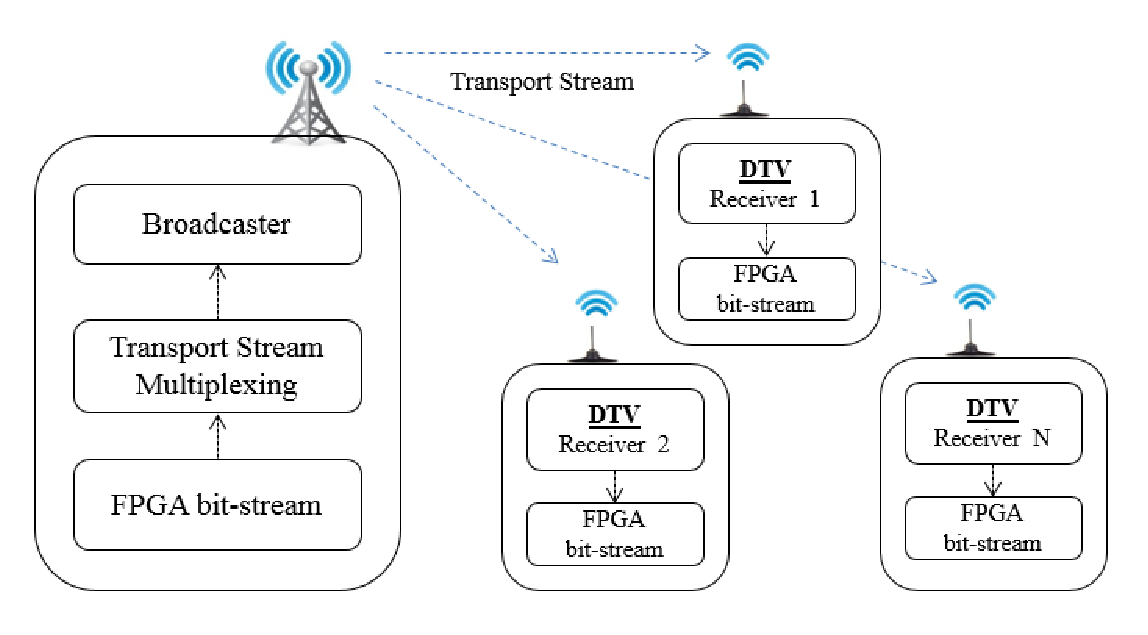
\includegraphics[width=2.5in]{images/Fig1.eps}
\caption{The FPGA bit-stream broadcast, in a DTV environment.}
\label{figure:fig1}
\end{figure}
%

This work deals with generic hardware update for DTV environments, where receivers do not need to leave the user premises. Indeed, designing reconfigurable hardware architectures can be an efficient way to improve the receiver lifespan, or even to create low cost receivers and embedded systems.

The presented scheme extends the use of DTV channels, introducing a way of transmitting synthesized hardware data. It can be employed in a wide range of future designs, regarding intelligent hardware architectures, and has the potential to boost the use of hardware reconfiguration in embedded solutions (e.g., DTV receivers), besides providing the opportunity to deeply exploit this scheme, in order to develop architectures to be reconfigured.

Hardware reconfiguration has already been used in a vast range of projects, but the solution presented here is an innovative way to perform this process. It is expected that the subject of this work, along with its related schema, can stimulate the scientific community to develop a wide range of environments, which rely on the hardware update technology.

The remaining of this work is organized as follows. Section \ref{related-work} provides a summary regarding the related literature. Section \ref{hardware-data} contains a brief explanation of DTV and data broadcasting. Next, section \ref{dtv-receiver} tackles reference receivers and basic concepts related to FPGA configuration schemes. Then, section \ref{hardware-reconfig} presents the complete hardware update approach, by detailing each step involved in this process. Finally, conclusions and future work are presented in section \ref{conclu}.


\section{Related Work}\label{related-work}

Recent studies, on similar topics, present some related work based on intelligent hardware architectures, with hardware reconfiguration, as the core technology for building more compact and efficient systems.
Indeed, architectures with hardware resource management present a new trend in embedded systems. In these approaches, pre-synthesized hardware unit functions are able to execute run-time reconfiguration of FPGA cores, according to the user's interaction, such as described by Lin {\em et al}~\cite{ref13}. \textcolor{red}{rodrigo, estenda a explicacao disso}

Intelligent embedded systems can make use of the partial dynamic hardware, for run-time reconfiguration. Such a feature, which is similar to a microprocessor multi-task system, allows a multiplex of distinct hardware modules to run at the same time. Thus, functional pre-synthesized hardware blocks, {\em i.e.}, logical blocks, can be reconfigured or not, according to system needs~\cite{ref14}. \textcolor{blue}{The associated system architecture is controlled by a microcontroller device, which is in charge of reconfiguring pre-synthesized hardware blocks, in the FPGA device. In addition, a list of pre-synthesized hardware blocks are kept in flash memory.} This way, the use of partial dynamic reconfiguration causes a considerable reduction in power consumption, besides a significant decrease in device costs.

The reconfigurable streaming architecture, presented by Hillenbrand {\em et al}~\cite{ref15}, allows the inclusion of signal-processing pre-synthesized cores, into hardware description language (HDL) sources, to be run-time reconfigurable. In that case, the pre-synthesized cores minimize the synthesis process and allow the design of adaptive reconfigurable system architectures. \textcolor{red}{rodrigo, estenda a explicacao disso}

A complete multi-core reconfigurable platform, combining processors with some reconfigurable logic, can provide a rich and flexible environment for application programmers, as proposed by Serres {\em et al}~\cite{ref16}. \textcolor{red}{rodrigo, estenda a explicacao disso}

\textcolor{red}{rodrigo, encontre pelo menos mais um trabalho e coloque aqui. Tente achar algo h�brido entre software e hardwareou qualquer outra coisa.}

The presented related works are based on pre-synthesized cores, which need to be present on their embedded file systems. Those cores are used according to system demands, or even due to user interaction. However, the proposed approach is based on broadcast networks, through which pre-synthesized cores, for updating several devices, can be sent. Therefore, several core modules, from different manufacturers, can be delivered at the same time, for a large amount of receivers.

\textcolor{blue}{Hardware reconfiguration techniques can be used in a wide variety of applications, in such a way that a specific feature can be updated or even integrated into a given platform, as seen above. Regarding video decoding, a similar result may be achieved with the reconfigurable video coding (RVC) framework \cite{ref34,ref40}, which provides coding specifications based on library components, instead of monolithic solutions. In summary, a coding problem can be tackled by selecting components of a standard coding-algorithm library, so that a specific solution may be assembled. Such an approach has the potential to even provide more flexibility on the choice of the coding-tool subset (profile), which already exists in current standards, given that it already presents some drawbacks, due to the lack of optimal solutions for many specific cases. The decoder model is provided via a specific language called Cal, which employs notions of actor programming and dataflow \cite{ref34,ref37}. There are also synthesis approaches \cite{ref37,ref35,ref36,ref39,ref41}, which are able to covert high-level descriptions to C or HDL code. Additionally, reconfigurable/multi-standard platforms \cite{ref38} can be developed, with the potential to reduce the hardware legacy problem.}

\textcolor{blue}{Based on what was presented, the relation between the proposed methodology and RVC can be analyzed from two different aspects. First, with an initial library of video coding-algorithms, an arbitrary combination of standardized basic coding algorithms can be obtained \cite{ref34}, which would provide optimal configurations for specific scenarios and indeed achieve the same goal of the proposed solution. The main difference here is that while RVC relies on a reconfiguration procedure regarding existing tools, the hardware reconfiguration would need a new hardware description to be transmitted; however, the latter has the potential to use less system resources ({\it e.g.,} memory and gates), when compared to RVC. In addition, receivers must be updated before receiving content coded with new algorithms, while RVC bit-streams carry all necessary information for decoding. Second, even that initial library will need to be updated, with new coding tools for enhanced performance or different coding paradigms. Thus, one may notice that the RVC framework and the proposed approach become complementary solutions, given that new modules could be generated and then transmitted and updated through the framework presented here. It is worth noticing that the mentioned synthesis tools \cite{ref35} can be used for generating a target decoder, based on the Cal description. Then, the resulting HDL module could be transmitted and used to update all available decoders, using the proposed methodology, in a similar way as in direct download applications \cite{ref34}.}


\section{Hardware-Data Broadcast Through The Digital TV Signal}\label{hardware-data}

The DTV TS consists of packets with audio, video, and data, which are $188$ bytes in length. The packet is the basic TS data unit and is composed of a sync-byte field, whose value is 0x47, followed by three $1$-bit fields (transport error indicator, payload unit start indicator, and transport priority) and an identification ($13$-bit), known as packet identifier (PID)~\cite{ref17}, among others. The PID provides a means of differentiating the payload content of each transport unit (packet), in a TS; if a PID is allocated and reported to a receiver (through a table), this means that a given packet carries video, audio, or other data, according to what was informed. Thus, the proprietary broadcast content is identified by its respective PID values.

Fig.~\ref{figure:fig2} shows a transport stream with different packets, which consist of video, audio, program association table (PAT), and hardware payload (PID 0x77). This transport stream slice shows that packets with the same PID, that is, carrying parts of the same information, are spaced over time. The receiver demultiplexer then needs to filter a transport stream, using the corresponding PIDs, for accessing its payload content.

%
\begin{figure}[ht]
\centering
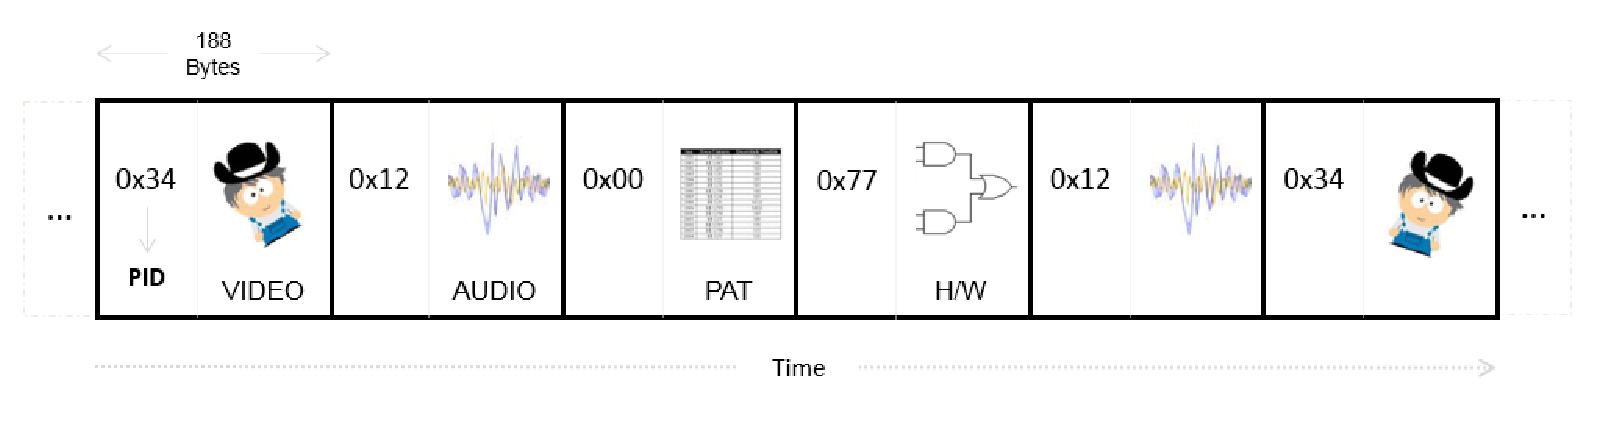
\includegraphics[width=3.5in]{images/Fig2.eps}
\caption{Transport stream packet structure used to carry different data types, which includes hardware reconfiguration data.}
\label{figure:fig2}
\end{figure}
%

The DTV system is able to broadcast binary applications~\cite{ref17}, which are interleaved with other HDTV contents (audio, video, and data). In order to inform that an application is being broadcast, the DTV standard uses the application information table (AIT)~\cite{ref18}. The AIT information is used, by the receiver resident system, for downloading all content related to the associated application.

The DTV telecommunication network allows the broadcast of several data types. Here, it is important to consider two main characteristics: the data format and the required synchronization, which are necessary for broadcasting some data types. The format may be classified into three categories, as follows: delimited data, un-delimited data, and datagrams following some protocol control. The delimited data can be divided into units of a defined size ({\em e.g.}, files and objects); however, the un-delimited data are considered continuous bit-streams. Finally, datagrams correspond to data packets related to a communication protocol ({\em e.g.}, IPv4 and IPv6).

Regarding synchronization, transmitted data are divided into synchronous, synchronized, and asynchronous~\cite{ref19}. The synchronous data have synchronization requirements with other data in the same stream, which is known as intra-media synchronization. Synchronized data are those that must be presented at predetermined time instances and in synchronism with elements of other media ({\em e.g.}, closed caption), which is called inter-media synchronization. Finally, the asynchronous data, in turn, have no temporal synchronization requirements. 

The data format characteristics and the required data synchronization are important to consider, when choosing the best way for data broadcasting.

\subsection{Data Broadcasting Mechanisms}\label{data-broadcasting}

An important feature of DTV standards is the data broadcasting capability. The broadcast data are normally used to describe and identify the HDTV broadcasted content. For instance, the European DTV standard, known as digital video broadcasting (DVB), offers four data transport mechanisms: data piping, data streaming, multiprotocol encapsulation (MPE), and Carousels~\cite{ref20,ref21}. Data piping is the simplest mechanism, which consists of inserting raw data directly into the TS packet payload area. Data streaming is more complex, when compared to the data piping method. The data streaming approach can arrange data using private sections or packetized elementary stream (PES) packets. Private sections are split into $4084$ bytes of payload, plus $8$ bytes of header and $4$ bytes of cyclic redundancy check (CRC), which amounts to $4096$ bytes. Some advantages regarding private sections are the contiguity control, given by the section number field and the error detection control, which is obtained via redundant information ({\em e.g.}, CRC\_32)~\cite{ref22}. Reimers describe the data streaming method by PES packets~\cite{ref23}. MPE uses the logical link control sub-network access protocol (LLC/SNAP) encapsulation, which allows for using any network protocol. Particularly, MPE allows for using unicast ({\em i.e.}, datagram sent to a single receiver) and multicast ({\em i.e.}, datagram sent to receiver sets). Carousels are techniques used to repeatedly deliver data in a continuous cycle ~\cite{ref24},~\cite{ref25}, as defined by the digital storage media command and control (DSM-CC) standard~\cite{ref26}, which is adopted by both digital audio video council (DAVIC) and DVB. DSM-CC specifies two types of carousels: data and object carousels. The latter extends the data carousel by specifying a file system directory structure ({\em e.g.}, media files, applications, image files, and directories). Section V-A addresses the presented broadcasting methods, by evaluating the core data characteristics and the most suitable method to implement hardware reconfiguration schemes.

\section{DTV Receiver Architectures and FPGA Reconfiguration Schemes}\label{dtv-receiver}

DTV receivers ({\em e.g.}, Set-top Boxes) are used to demodulate and decode the HDTV broadcast signal, in such a way that the transmitted TS, carrying audio, video, and data packets (see section \ref{hardware-data}) is recovered. Normally, DTV standards specify reference receiver architectures, in order to suggest design implementations to manufacturers~\cite{ref27}. In fact, commercially available receivers normally present similar composition and provide a set of device drivers with exemplary applications. These data are taken as a reference to access and manipulate hardware devices. 

Fig.~\ref{figure:fig3} shows the basic components present in receiver architectures. The air interface ({\em e.g.}, front-end, also called demodulator) device is responsible for demodulating any available DTV signal, in the receiver range. It recovers the TS stream flow output by the multiplexer device, which was sent at the transmitter end. The DEMUX component uses the front-end (air interface) output (a transport stream flow), splits packets related to a given PID identifier (see section \ref{hardware-data}), and outputs them in continuous separate flows. Later on, those flows are forwarded to their respective decoders ({\it e.g.}, H.$264$ video decoder), which in turn decode the content ({\em e.g.}, audio or video packets), in a continuous decoding process. \textcolor{blue}{Finally, the information output by the video decoder is passed to its respective digital video encoder (DENC) module, which converts digital baseband video data into analog signals ({\it e.g.}, Y/C and composite video broadcast signal), in order to provide video interface with other equipment ({\it e.g.}, television sets and personal video recorders)}. The other flows, present in the transport stream, are split by DEMUX, according to a given PID provided by the resident application ({\em e.g.}, filter software parser) control.

%
\begin{figure}[ht]
\centering
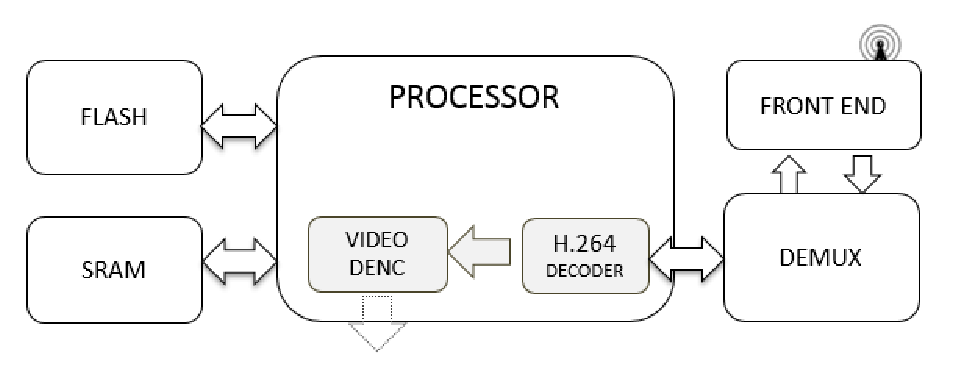
\includegraphics[width=2.5in]{images/Fig3.eps}
\caption{Receiver architecture composed of air interface (Front End), demultiplexer, H.264 decoder, and memories.}
\label{figure:fig3}
\end{figure}
%

\subsection{FPGA Standalone Reconfiguration Schemes}\label{fpga-standalone}

The standard process of hardware development begins with a design entry ({\em e.g.}, hardware schematics or HDL)~\cite{ref28}. Then, a HDL is used for developing hardware specifications to configure a FPGAs or a complex programmable logic device (CPLD). The most well-known HDLs are VHDL and Verilog. In the final step of the design flow, a bit-stream file ({\em e.g.}, raw binary file - RBF) is generated, which is then used to reconfigure the FPGA device. Typically, it is done by an electronic design automation (EDA) tool, which is also provided by the FPGA manufacturer~\cite{ref28}. Thus, it is possible to validate the final design behavior before delivering the bit-stream.

Although the FPGA reconfiguration is done by a tool, typically provided by the manufacturer, one may also develop a standalone reconfiguration scheme. In general, standalone schemes employ two modes ({\em e.g.}, master or slave modes) to reconfigure the FPGA, using a bit-stream (pre-synthesized binary code). In master mode, an FPGA is typically used to control the reconfiguration process; however, in slave mode, the FPGA configuration is controlled by an external device ({\em e.g.}, microcontroller, CPLD, or another FPGA). Additionally, the standard IEEE $1149.1$~\cite{ref29}, known as joint test action group (JTAG), is another mode commonly used by FPGA manufacturers. Normally, FPGA manufacturers provide a JTAG cable along with a programming tool, which is used to reconfigure their FPGA development boards. These cables are available to work with different communication interfaces, such as USB, Parallel/Serial port, or Ethernet, and are an attractive way to construct a host/target communication interface. This interface is commonly adopted by several embedded systems and has already been largely tested and validated. The JTAG has basically $4$ control signals: test data input (TDI), test data output (TDO), test mode select (TMS), and test clock (TCK), which are used to configure the device through a test access port (TAP) controller~\cite{ref29}. 

The literature also presents standalone open-source JTAG libraries~\cite{ref30},~\cite{ref31} that enable a variety of JTAG-based manufacturer communication cables. Those libraries can use the serial vector format (SVF)~\cite{ref32}, to configure several FPGA models. The SVF file, which describes actions over JTAG interfaces, is a standard used for exchanging descriptions of high-level IEEE 1149.1 (JTAG) bus operations~\cite{ref32}. The standalone program can parse and play the SVF file, thus reconfiguring the FPGA.

SVF files can be obtained from other formats, through a converting tool or even an FPGA manufacturer tool. Indeed, most FPGA manufacturers commonly provide this file, which is used as a standard format to reconfigure devices.

In order to create a host/target physical connection, the reference DTV receiver was used as host device, and a commercial FPGA board as target device. The USB-manufacturer programmer cable, based on the JTAG program mode, is used to connect both sides, as seen in Fig.~\ref{figure:fig4}.

The standalone FPGA programmer system was based on an open-source JTAG reference code, which was adapted to fit the DTV receiver ({\em i.e.}, the module responsible for reconfiguring the FPGA). In order to do that, some third-party libraries were integrated to the receiving system, so that the open-source code could work properly. Thus, the resident application (reconfiguration module) is able to control the FPGA-board read and write (R/W) operations.

%
\begin{figure}[ht]
\centering
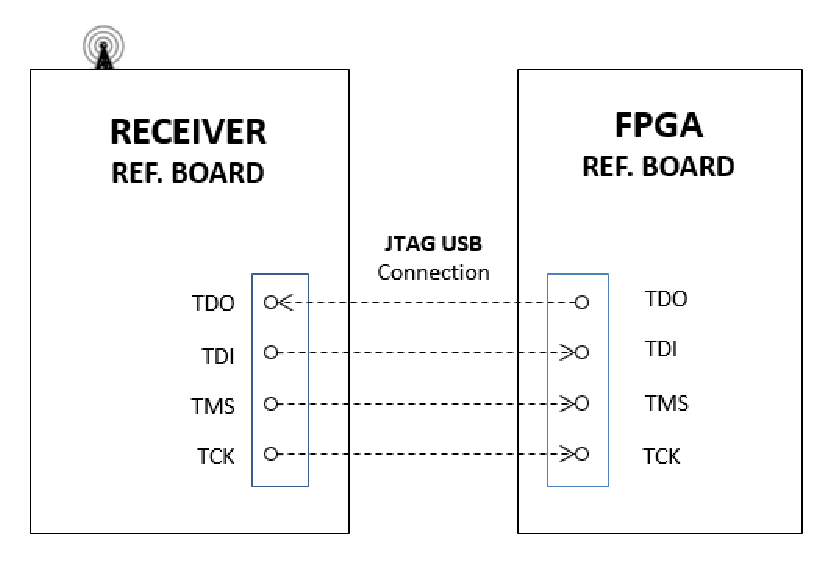
\includegraphics[width=2.5in]{images/Fig4.eps}
\caption{The DTV Receiver (host) connected to a reference FPGA board (target), through a USB/JTAG programmer cable.}
\label{figure:fig4}
\end{figure}
%

\section{The Hardware Reconfiguration Scheme Based on the DTV Signal}\label{hardware-reconfig}

The entire hardware reconfiguration scheme can be split into three distinct steps. The first consists of preparing data to be broadcast. In particular, that means encapsulating the synthesized FPGA bit-stream into a transport stream. Here, it is assumed that the bit-stream is already synthesized, tested, and validated for the same FPGA model used by the receiver. The second step involves filtering, remounting, checksum validation, and persistence. Finally, the final step uses the downloaded bit-stream to reconfigure the receiver FPGA module. All mentioned steps, which results in the complete reconfiguration process of the FPGA device compose the proposed scheme. The following sections discuss each procedure step, in detail.

\textcolor{blue}{\subsection{Encapsulating Hardware data}
\label{encap-method}
In order to choose a transmission method for hardware reconfiguration modules, one must take into account data format and timing requirements. Regarding data format, the possible classifications are: delimited, undelimited, and datagrams. Delimited data can be divided into units with a given size, like objects, files, etc. Undelimited data, in turn, are considered continuous bit flows. Finally, datagrams consist in fragmenting data into packets, which is followed by a communication protocol. When addressing timing requirements, data can be synchronous, synchronized, and asynchronous. Synchronous data present timing links with other data on the same stream, which is commonly know as intra-media synchronization. Synchronized data must be presented in predetermined time instants and according to elements of other media, such as video or audio, which is commonly know as inter-media synchronization. Asynchronous data, in turn, do not present any timing requirements.  Table \ref{table:table-one} shows a summary of what was tackled here, regarding the data broadcasting mechanisms presented section \ref{data-broadcasting}.}

\textcolor{blue}{\begin{table}[ht]
\renewcommand{\arraystretch}{1.18}
\begin{center} {\small
\caption{Comparison Regarding Data Broadcasting Methods}
\label{table:table-one}
\centering
\begin{tabular}{| >{\centering}m{1.2cm} >{\centering}m{1cm} >{\centering}m{0.9cm} >{\centering}m{1cm} >{\centering}m{0.6cm} c|}
\hline\hline
  & & &  \multicolumn{2}{c}{Data Streaming} & \\ 
   \multicolumn{2}{|c}{Requirements}
  						& Data Piping 	& Private Section 	& PES 	& Carousel\\
\hline\hline
\multicolumn{2}{|c}{Support to error detection} 
						& {|} 			& OK 			& OK 	& {|}\\
\multicolumn{2}{|c}{Support to broadcast} 
						& OK 		& OK 			& OK 	& OK\\
						& & & & &\\
Support & Synchronous		& {|} 			& {|}	 			& OK 	& {|}\\
unbounded & Asynchronous	& OK 		& OK 			& {|}	 	& {|}\\
Data & Synchronous			& {|}			& {|}	 			& OK 	& {|}\\
						& & & & &\\
Support & Synchronous		& {|} 			& {|}	 			& {|}	 	& {|}\\
unbounded & Asynchronous	& {|} 			& OK 			& {|}	 	& OK\\
Data & Synchronous			& {|}			& {|}	 			& {|}	 	& OK\\
\hline\hline
\end{tabular} }
\end{center}
\footnotesize{``OK'' means appropriate method and ``-'' means no support or not appropriate.}
\end{table}}

\textcolor{blue}{Ultimately, hardware cores are binary data, which contain hardware descriptions for configuring FPGA devices. This way, the hardware reconfiguration stream is regarded as delimited data and can be divided into slices of predetermined size. Moreover, it does not have temporal requirements and can be considered asynchronous data.}
%

\textcolor{blue}{Indeed, the biggest concern lies on the data recovery procedure, which must be reliable and provide error-correcting capability. Using carousels \cite{ref20,ref21}, there is infrastructure regarding data recovery; however, they use complex structures, which incur larger overhead and high computational effort. MPE can not be considered, due to its dependence on a network protocol, and data piping does not provide synchronization capability. Besides, hardware reconfiguration files are not very big, which suggests simple transport mechanisms. As a consequence, a good option is the data streaming through private sections approach, which is simple and already provides error-detection tools and support to delimited and asynchronous data, with structures less complex than the ones used in carousels. In summary, the reconfiguration file can be partitioned in sections, which are enumerated according to their insertion order and cyclically repeated, as shown in Fig. \ref{figure:figcyc}.}

\textcolor{blue}{\textcolor{red}{Rodrigo, coloque a figura em ingles}
\begin{figure}[ht]
\centering
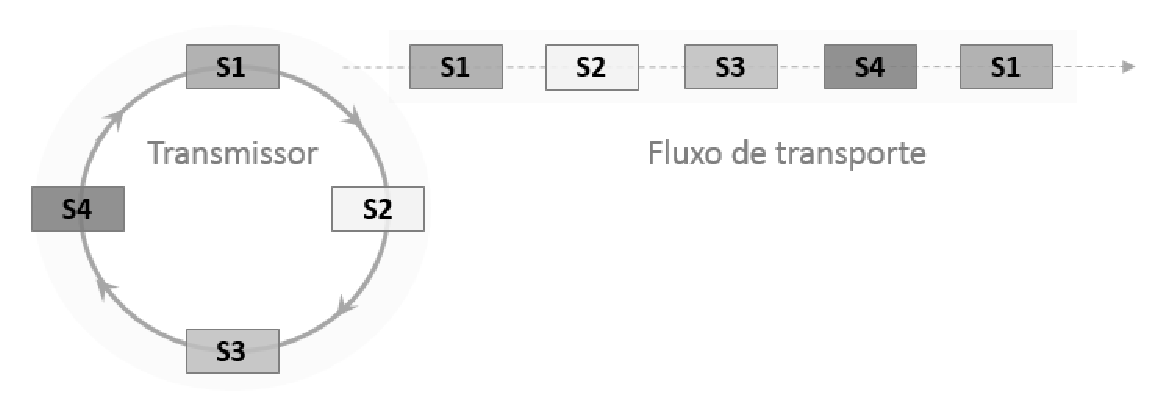
\includegraphics[width=3in]{images/cyc.eps}
\caption{Transmission strategy with private sections.}
\label{figure:figcyc}
\end{figure}}

\subsection{Hardware Data Multiplexing in Transport Streams}\label{data-multiplexing}
\textcolor{blue}{From the point of view of the DTV signal, the FPGA bit-stream is seen as regular data. This way, such content needs to be signaled ({\em i.e.}, a PID to identify the content flow and description information, using a new data table), in order to notify the receiver about its existence, in the broadcast signal.}

\textcolor{blue}{In order to add information regarding that, one must follow the DTV standard rules. First, it is necessary to choose a suitable method for transporting reconfiguration bit-streams, by taking into account their main characteristics, which was done and led to data streaming through private sections (see section \ref{encap-method}).}



%Beyond what was tackled, other criteria for choosing the most suitable data broadcast method were taken into consideration: support for error detection and capability to perform broadcast. TABLE~\ref{table:table-one} compares the data piping, data streaming and carousel techniques, in order to check the most suitable method for this task. MPE was not considered here, due to its dependence on a network protocol (see section \ref{data-broadcasting}). Considering what is shown in TABLE~\ref{table:table-one}, the most appropriate data broadcasting method, for transporting hardware reconfiguration data, is data streaming using private sections.


Thus, the hardware bit-stream is divided into sections of $4092$ bytes in length, as illustrated in Fig.~\ref{figure:fig5}, according to the data streaming rules. The identification of the private section content is given by $table\_id$, which is an $8$-bit field of the private section table. The $section\_number$ field presents the sequential number of a section, which is used to keep the correct order for data remounting. It is worth noticing that sections can arrive out of order and, therefore, the resident receiver system needs to implement a mechanism to maintain the correct section order.

%
\begin{figure}[ht]
\centering
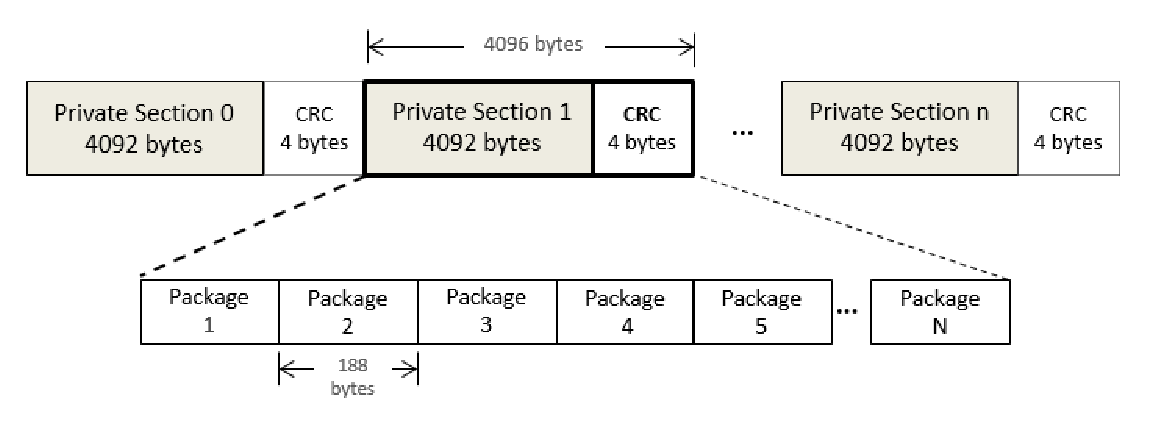
\includegraphics[width=3in]{images/Fig5.eps}
\caption{The FPGA synthesis stream, divided into sequenced private sections of variable size, which are then organized into TS packets.}
\label{figure:fig5}
\end{figure}
%

The $last\_section\_number$ field indicates the total number of sections used for carrying the synthesized hardware content. The $private\_data\_byte$ field is a variable size one, which is used to carry the FPGA bit-stream. 

For this work, the $section\_syntax\_indicator$ field was set to `1', in order to enable the CRC\_32 checksum field of the private section syntax. This redundant information enables the receiver to detect errors, via a checksum algorithm.

In order to signal the FPGA bit-stream content, the proposed scheme follows a syntax similar to the one used by AIT. In summary, it must provide a FPGA bit-stream description and an access point, in such a way that the receiver is able to download and remount FPGA core data. The new table, named update information table (UIT), follows the AIT syntax. Its role is to provide detailed information about characteristics of the transmitted FPGA core. This is crucial information used by the receiver, in order to decide if the transmitted content can be used or not. The FPGA core information, borne by the new table, is then used by the receiving device, in order to filter the hardware bit-stream.

Other information, about the transmitted hardware core, must also be included and broadcast, along with hardware contents, such as a description of the hardware upgrade module ({\em e.g.} decoder, multiplexer, cypher, etc.), FPGA manufacturer name, family, device part number (which was used to synthesize the core), size of the synthesized core, in bytes, PID and TID for section filtering, etc. The mentioned data need to be added to the TS, in order to provide all necessary information related to the new content. TABLE~\ref{table:table-two} shows the complete UIT structure, whose mnemonics are define in the MPEG-2 systems standard~\cite{ref17}.

\begin{table}[ht]
\renewcommand{\arraystretch}{1}
\begin{center} {\small
\caption{The Update Information Table - UIT}
\label{table:table-two}
\centering
\begin{tabular}{|>{\flushleft}m{3.8cm} >{\centering}m{1.3cm} >{\centering}m{1.2cm} c |}
\hline\hline
Data Structure 				& Bit Rate (No. of bits) 	& Mnemonic 	& Value\\
\hline\hline
update\_information\_table() \{	& 					&			&		\\			
table\_id					& 8					&	uimsbf	& 0x91	\\
section\_syntax\_indicator		& 1  					&	bslbf		&		\\	
hw\_core\_flag				& 1					&	bslbf		&		\\
Reserved					& 2					&	bslbf		&		\\
section\_lenght				& 12					&	uimsbf	&		\\
fpga\_core\_number			& 16					&	uimsbf	&		\\
Reserved					& 2					&	bslbf		&		\\	
version\_number			& 5					&	uimsbf	&		\\
current\_next\_indicator		& 1					&	bslbf		&		\\
section\_number			& 8					&	uimsbf	&		\\
last\_section\_number		& 8					&	uimsbf	&		\\
reserved\_future\_use		& 4					&	uimsbf	&		\\
update\_loop\_lenght			& 12					&	uimsbf	&		\\
for (i=0; i \textless N; i++) \{	&				 	&			&		\\			
descriptor()				& 					&			&		\\	
\}						& 					&			&		\\
reserved\_future\_use		& 4					&	bslbf		&		\\
update\_loop\_length			& 12					&	uimsbf	&		\\
for (i=0; i \textless N; i++) \{	&				 	&			&		\\	
update\_hw\_identifier() 		& 					&			&		\\	
reserved\_future\_use		& 8					&	uimsbf	&		\\
reserved\_future\_use		& 4					&	bslbf		&		\\
descriptors\_loop\_length		& 12					&	uimsbf	&		\\
for(i=0; i \textless N; i++) \{ 	&				 	&			&		\\
descriptor() 				& 					&			&		\\
\}						& 					&			&		\\
\} 						&				 	&			&		\\
CRC\_32 					& 32					&	rpchof	&		\\
\}						& 					&			&		\\
\hline
\end{tabular} }
\end{center}
\end{table}

Program map table (PMT) sections provide the access point to the newly created UIT table, in a similar way as already done for AIT. UIT gives access to the $hw\_core\_flag$ field, which is used to signal the existence of hardware content. If this field is set to `0x1', this means that there is hardware content in the DTV signal; otherwise, `0x0' indicates that no hardware content is being broadcast.

The $fpga\_core\_number$ field identifies the number of hardware cores being currently broadcast. The other necessary data are provided by $update\_hw\_identifier()$, which is a specific descriptor regarding transmitted hardware modules, similar to $application\_identifier()$, used in AIT. The $update\_hw\_identifier()$ portion presents a list of available hardware cores, whose size was reported by $fpga\_core\_number$. The syntax of $update\_hw\_identifier()$ is shown in TABLE~\ref{table:table-three}.

\begin{table}[ht]
\renewcommand{\arraystretch}{1}
\begin{center} {\small
\caption{The update\_hw\_identifier Field Syntax}
\label{table:table-three}
\centering
\begin{tabular}{|>{\flushleft}m{3.8cm} >{\centering}m{1.3cm} >{\centering}m{1.2cm} c |}
\hline\hline
Data Structure 				& Bit Rate (No. of bits) 	& Mnemonic 	& Value\\
\hline\hline
update\_hw\_identifier () \{		&					&			&	     \\			
fpga\_core\_size			& 32					& bslbf		&	     \\
fpga\_core\_version			& 16					& bslbf		&	     \\
fpga\_core\_module\_name()	&					&			&	     \\		
fpga\_core\_device\_info()		&					&			&	     \\	
fpga\_section\_identifier()		&					&			&	     \\	
\}						&					&			&	     \\
\hline
\end{tabular} }
\end{center}
\end{table}

The $fpga\_core\_size$ filed is $32$ bits in length, informs the core size, and is used by the receiver application, in order to check if the whole bit-stream content was reassembled. The $fpga\_core\_version$ field identifies the core update version number and is used during the reassembling process, in order to check if the receiver was already updated. The following three fields are descriptors, which bear information about each transmitted core. In addition, there is a list of access points (PID and TID), which are used for filtering private sections carrying hardware-reconfiguration content (see TABLE~\ref{table:table-four}). 

TABLE~\ref{table:table-four} presents the syntax of the $fpga\_core\_module\_name()$ descriptor, which is identified by a $descriptor\_tag$ set to `0x01'. 

\begin{table}[ht]
\renewcommand{\arraystretch}{1}
\begin{center} {\small
\caption{The FPGA\_core\_module\_name Descriptor Syntax}
\label{table:table-four}
\centering
\begin{tabular}{|>{\flushleft}m{3.8cm} >{\centering}m{1.3cm} >{\centering}m{1.2cm} c |}
\hline\hline
Data Structure 				& Bit Rate (No. of bits) 	& Mnemonic 	& Value\\
\hline\hline
fpga\_core\_module\_name() \{	&					&			&	     \\		
descriptor\_tag				& 8					& uimsbf		& 0x01  \\		
descriptor\_lenght			& 8					& uimsbf		&	     \\		
for(i=0; i \textless N; i++)\{		&					&			&	     \\	
reserved\_future\_use		& 24					& bslbf		&	     \\		
descriptor\_core\_length		& 8					& uimsbf		&	     \\		
for(i=0; i \textless N; i++) \{	&					&			&	     \\		
  fpga\_core\_module\_name	& 8					& uimsbf		&	     \\		
\}						&					&			&	     \\
\}						&					&			&	     \\
\}						&					&			&	     \\
\hline
\end{tabular} }
\end{center}
\end{table}

The descriptor\_length field identifies the size of the content located inside the loop. The next field, that is, descriptor\_core\_length, identifies the size of the fpga\_core\_module\_name information, which is composed by 32 characters, where each one is coded with 8 bits. Such a field is used to inform the hardware module name (e.g. decoders, multiplexer, cypher, etc.) available for reconfiguration. The next descriptor is named fpga\_core\_device\_info()  and is shown in TABLE~\ref{table:table-five}. This descriptor is identified by a descriptor\_tag set to `0x03'. Its descriptor\_length field presents the size of the fpga\_info string field, where each character is also coded with 8 bits. This field informs the name of the FPGA manufacturer, followed by the FPGA family and, lastly, the part number of the FPGA device, for which the core was synthesized. Such values are arranged into the fpga\_info character string field, separated by spaces (`0x32'): ``fpga-manufacturer-name fpga-family-name fpga-part-number''. This information is used, by the receiver, to identify the FPGA device information in the broadcast content.

\begin{table}[ht]
\renewcommand{\arraystretch}{1}
\begin{center} {\small
\caption{The FPGA\_core\_device\_info Descriptor Syntax}
\label{table:table-five}
\centering
\begin{tabular}{|>{\flushleft}m{3.8cm} >{\centering}m{1.3cm} >{\centering}m{1.2cm} c |}
\hline\hline
Data Structure 				& Bit Rate (No. of bits) 	& Mnemonic 	& Value\\
\hline\hline
fpga\_core\_device\_info() \{	&					&			&	    \\		
descriptor\_tag				& 8					& uimsbf		& 0x03 \\
descriptor\_length			& 8					& uimsbf		&	    \\	
for(i=0; i \textless N; i++)\{		&					&			&	    \\
fpga\_info					& 8					& uimsbf		&	    \\	
      \}						&					&			&	    \\
\}						&					&			&	    \\
\hline
\end{tabular} }
\end{center}
\end{table}

The last descriptor is the fpga\_section\_identifier(), shown in TABLE~\ref{table:table-six}. This descriptor is identified by a descriptor\_tag set to `0x05'. The next field, that is, descriptor\_length, contains the loop content size, in bytes. The remount\_core\_pck\_pid field informs the PID used to locate packets with the desired hardware content. Besides, it is used, in association with the remount\_core\_sec\_tid field (which informs the section table ID (TID)), for accessing private sections with core content. The remount\_priority field informs the remount priority order for each group of $256$ sections, represented by its own PID and TID. Such an approach is used if the hardware bit-stream needs more than $256$*$4080$ bytes; otherwise, only one group is enough, that is, it is set to `0x00'. For the next group represented by other PIDs and TIDs, this value is incremented by $1$ and so on. 

The receiver system uses the presented information to check the characteristics of the broadcast hardware core and, if a match is found, to guide the execution of hardware updates.

\begin{table}[ht]
\renewcommand{\arraystretch}{1}
\begin{center} {\small
\caption{The FPGA\_section\_identifier Descriptor Syntax}
\label{table:table-six}
\centering
\begin{tabular}{|>{\flushleft}m{3.8cm} >{\centering}m{1.3cm} >{\centering}m{1.2cm} c |}
\hline\hline
Data Structure 				& Bit Rate (No. of bits) 	& Mnemonic 	& Value\\
\hline\hline
fpga\_section\_identifier() \{	&					&			&	    \\		
descriptor\_tag				& 8					& uimsbf		& 0x05 \\
descriptor\_lenght			& 8					& uimsbf		&	    \\	
for(i=0; i \textless N; i++) \{	&					&			&	    \\		
remount\_core\_pck\_pid		& 32					& bslbf		&	    \\	
          remount\_core\_sec\_tid	& 16					& bslbf		&	    \\	
remount\_priority			& 8					& uimsbf		&	    \\	
\}						&					&			&	    \\
\}						&					&			&	    \\
\hline
\end{tabular} }
\end{center}
\end{table}


\subsection{Core Data Filtering}\label{core-data}

The DTV-receiver resident system is configured to filter the transmitted content, in order to find some hardware reconfiguration bit-stream (core). The system will look for UIT and parse it, beginning with the $hw\_core\_flag$ field. If it is set to `0x0', the system simply ignores the current UIT; otherwise (`0x1'), there is a signaled hardware bit-stream content and the system then parses the remaining UIT content ({\em e.g.}, $fpga\_core\_size$, $fpga\_core\_version$, $fpga\_core\_module\_name$, etc.), in order to retrieve the corresponding table fields, which describe the characteristics of the broadcast bit-stream (hardware core). Finally, such values are compared with the suitable FPGA, as shown in Fig.~\ref{figure:fig6}. The characteristics of the suitable FPGA device can be stored in a simple text file, which is made available at the receiver file system, as done here.

%
\begin{figure}[ht]
\centering
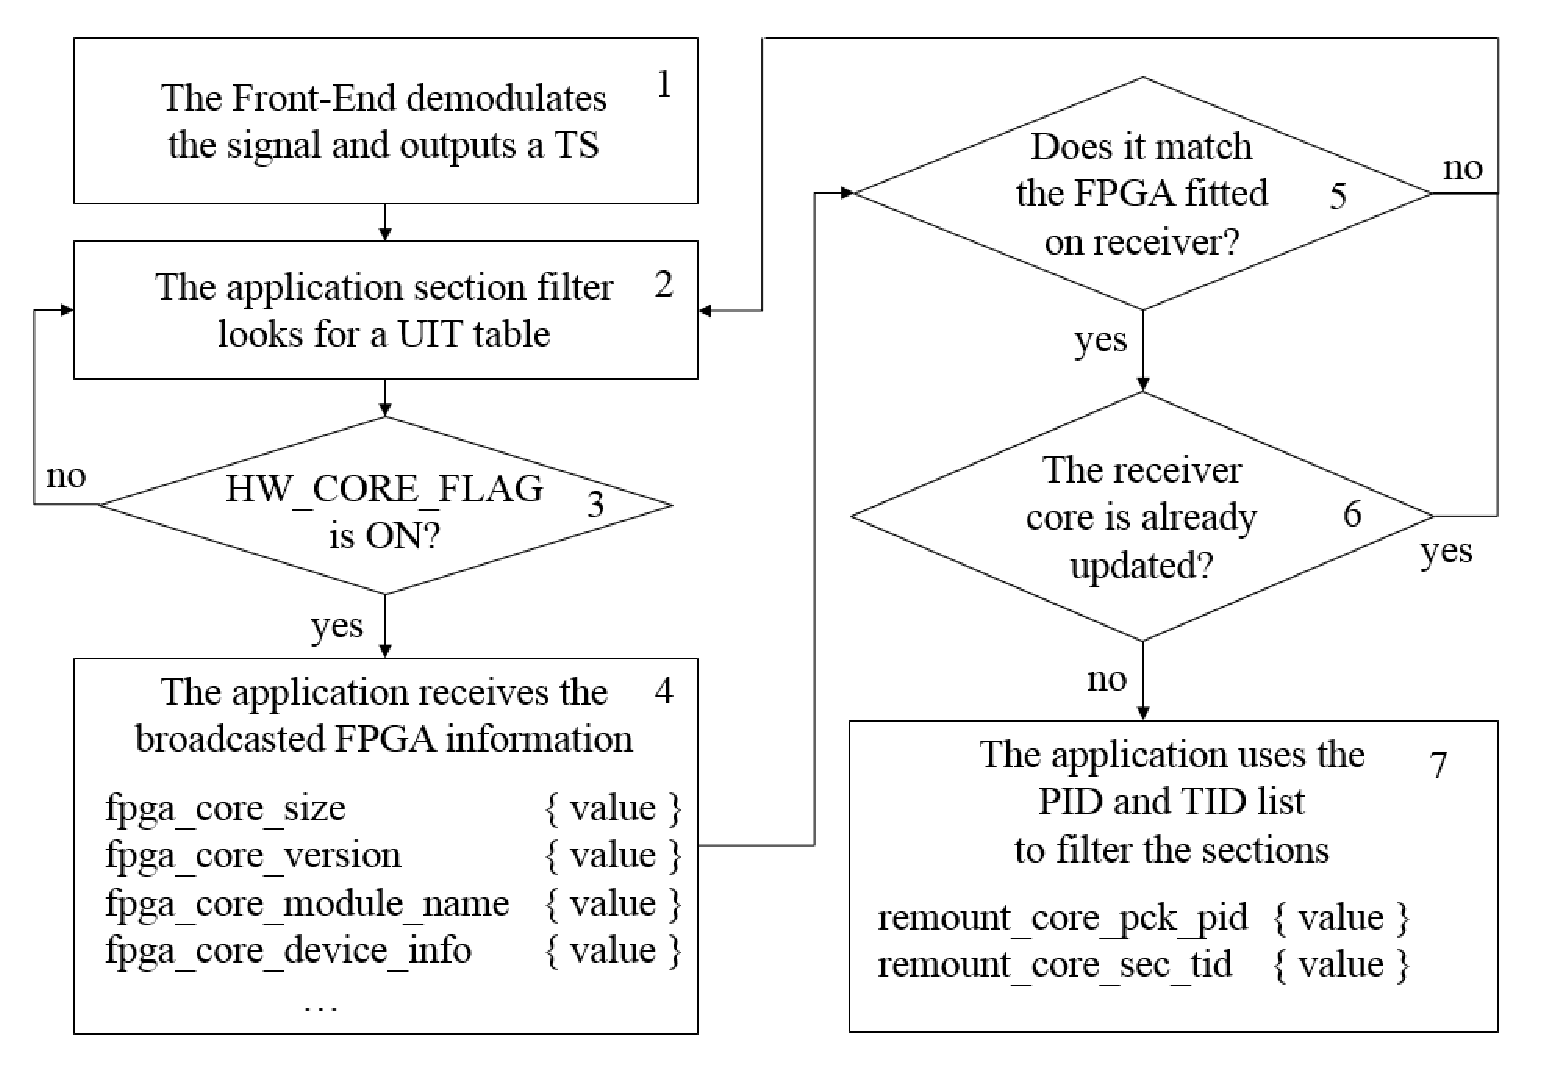
\includegraphics[width=2.5in]{images/Fig6.eps}
\caption{Steps to check the UIT content and find a broadcast core hardware suitable for the receiver, in order to retrieve the correct PID for filtering.}
\label{figure:fig6}
\end{figure}
%

If some of these fields do not match the receiver hardware characteristics, the system then interrupts the reconfiguration process. Indeed, it may happen, given that content may have been sent to another kind of receiver, with different FPGA devices. On the other hand, if this content fits the receiver hardware architecture, then the system continues the filtering procedure and parses the $remount\_core\_pck\_pid$ and $remount\_core\_sec\_tid$ fields. Those values are used as an access point for extracting the transmitted reconfiguration bit-stream (for programming section-filter modules), directly from private sections, as depicted in Fig.~\ref{figure:fig7}. When a private section is retrieved, its CRC is checked, for validation purposes (see section \ref{data-broadcasting}). If the section is not corrupted, the system stores the section payload, according to the section order provided by the $section\_number$ field. 

The system keeps this iterative process until the last section is received, in order to conclude the reassembling process. However, the procedure completion depends on the validation of the entire private section payload. If a section is not validated ({\em e.g.}, corrupted), the reconfiguration process discards that and the search for a valid section content continues. Given that sections may be randomly retrieved, the receiving system is responsible for ensuring correct order.

%
\begin{figure}[ht]
\centering
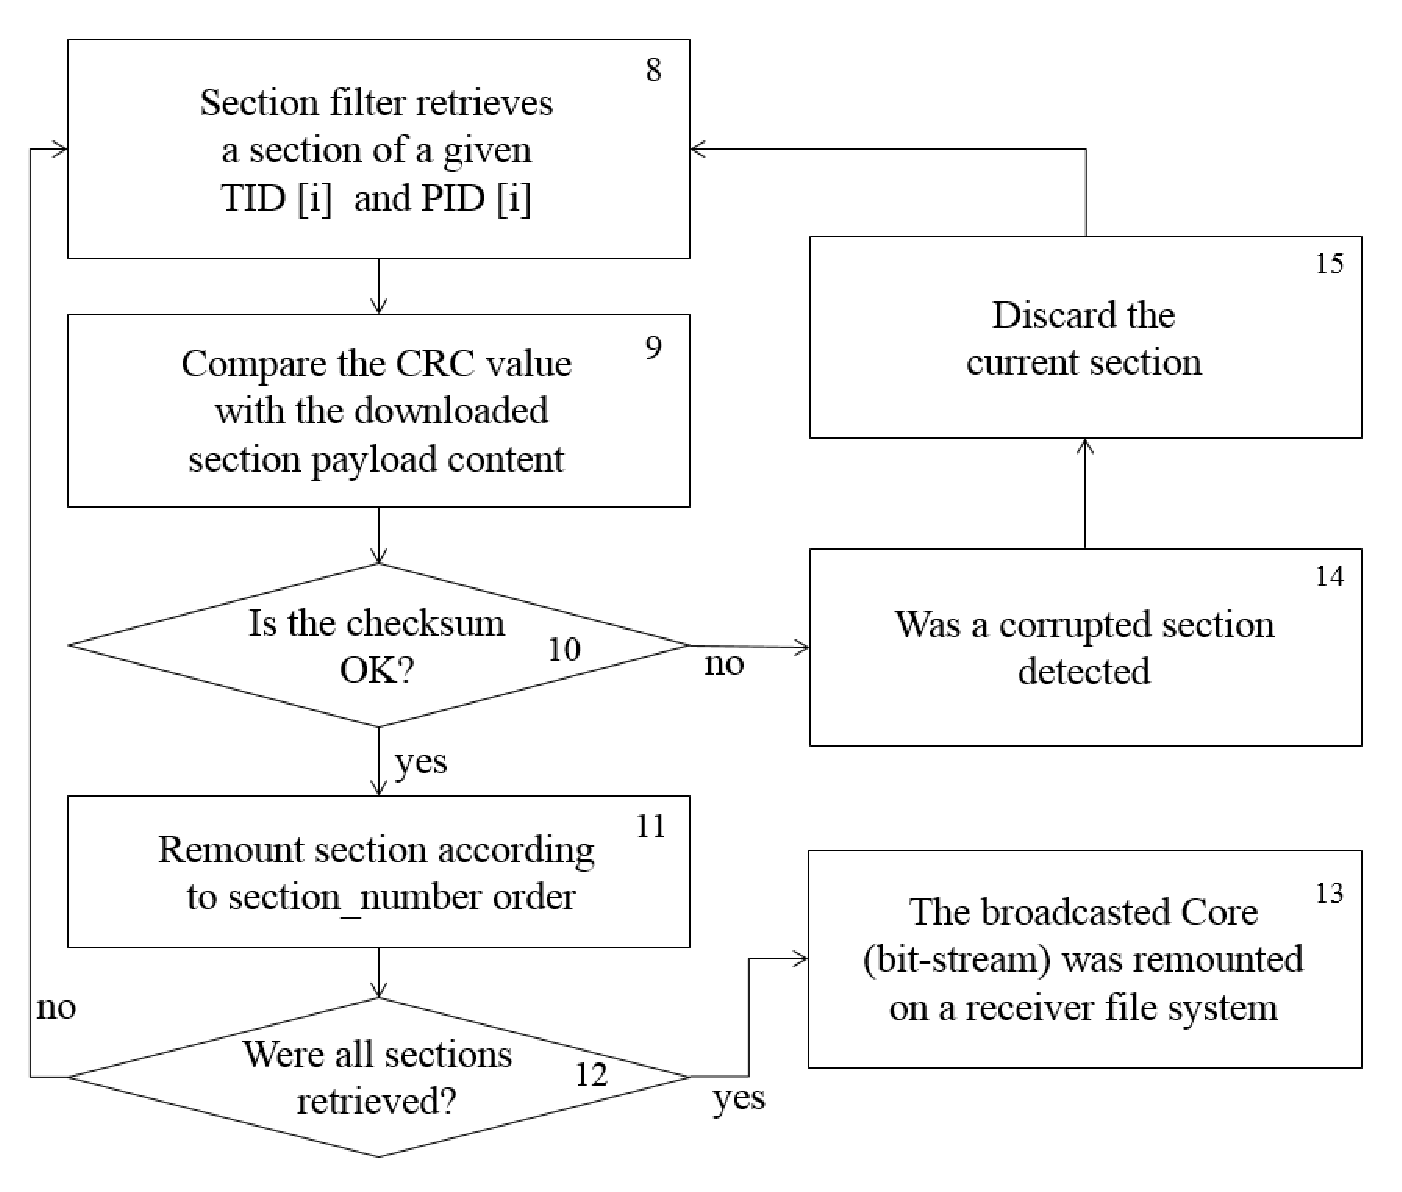
\includegraphics[width=2.5in]{images/Fig7.eps}
\caption{Steps involved in the process of obtaining the broadcast hardware core stream, which includes verification of each private section, downloading and content reassembling.}
\label{figure:fig7}
\end{figure}
%

\subsection{The Target Device Reconfiguration}\label{target-device}

The FPGA reconfiguration is the last step of the entire proposed scheme. The main idea is to exercise the complete chain, that is, from the beginning of the process (core multiplexing) to its end (FPGA reconfiguration). At this point, the receiver has already checked if the core characteristics fit the FPGA model (see section \ref{core-data}), used at the receiver, and has finished the system core reassembling (obtained broadcasted SVF file). Now, in this step, the remounted hardware core stream reaches a receiver reconfigurable target device, through a JTAG mode, as presented in section \ref{data-multiplexing}. 

\textcolor{red}{Rodrigo, aqui voce criarah uma nova subsecao de discussao, onde voce falarah que usando jtag, svf e as tabelas, onde informacoes sobre o FPGA sao disponibilizadas (fabricante, etc,.), a metodologia n�o fica limitada a um fabricante especifico... (eh isso, nao eh?)... voce tamb�m refor�ar� que se o feixe de bits nao for compativel, nada acontecerah...Aqui fale do quanto de informacao, alem da descricao de hardware, foi necessario para o processo de reconfiguracao... por exemplo, comandos de jtag... fale quanta informacao eh necessario alem da descricao propriamente dita... fale tambem que a metodologia proposta necessita de mudancas no padrao, entretanto, isso viabilizaria um esquema consistente e bem formatado para atualiza��o... fale tambem de seguranca... e fale que o FPGA deve prever algoritmos mais complexos que o atual... mais poder de processamento... deixe tudo em azul}

\subsection{System Compatibility}\label{system-compatibility}

\textcolor{blue}{This scheme allows to broadcast content for different models of FPGAs from several manufactures. The strategy used to signalize the details of the transported core, through UIT table multiplexed with the transport stream allows to describe the details of diferentes FPGA (e.g., FPGA manufacturer, FPGA Family, FPGA part number, FPGA core size, etc). Thus, the receivers can fit any FPGA in their hardware architectures. The receiver is able to select the transport content broadcast for its own architecture only. It is possible because the system crosses the signalization data (e.g., description of FPGA target for which the core was synthetized) provided by UIT table with the FPGA fitted on receiver architecture. Thus the system manage the discard or the use of the bitstream. During the bitstream reassembling, the system check and validate each payload of the private section in order to check if there is corrupted data. It is performed through a checksum with the received data with the CRC value broadcasted with each private section data. Thus when some corrupted section is detected the system will discard this section and wait for a new one in the next cycle. 
The scheme is also compatible with any proprietary FPGA bitstream format. The use of proprietary formats reconfiguration files present low overhead during the FPGA reconfigurantion process. In this case, for each FPGA model, is necessary a dedicated programing mode. For the other side, the use of standard formats, such as, SVF file format presents more overhead during the reconfiguration process because this format include the JTAG commands to program the FPGA. JTAG is a well known data exchange interface is largely used for electronic devices and IC devices including the FPGA.}
\textcolor{red}{Ainda n�o finalizei s� inclu� para bckup... Eddie se quiser ver se at� aqui � mais ou menos o que vc espera.. pode incluir seus comments.. Vou ter que sair as 17:00 daqui... }

\textcolor{red}{O texto abaixo ja faz parte da explicacao da mudanca na norma}

\textcolor{blue}{One may notice that the proposed methodology is based on an extension of the current service information (SI) standards \textcolor{red}{aqui vai uma ref de SI}, without any modification w.r.t. current structures, since it uses a new table (UIT) and associated descriptors. Although that may sound complicated, its implementation is transparent and can even be done without a formal modification of the related standards, as a proprietary framework. Apart from that, the present approach addresses the complete update chain and provides an elegant and complete solution, which is still more feasible and simpler than isolated proprietary solutions or on-site maintenace.}

\subsection{Reconfiguration-Process Test Results}\label{reconfig-process}

As Proof of Concept (PoC), some HDL source code examples were synthesized, which aim at exciting the entire scheme. Fourth VHDL/Verilog source code examples are used, which are synthesized for a reference FPGA and then tested and validated, by means of an EDA tool.

\textcolor{red}{Rodrigo, aqui voce coloca um resumo do seu ambiente de testes, com placa de FPGA, frequencia da placa, computador, etc. coloque tudo que voce usou e deixe em azul}

The validation is based on typical examples, in order to check if the FPGA is configured properly and the scheme works in a DTV system. The first pre-synthesized example converted to an SVF file (see section \ref{hardware-data}) is a simple binary-coded decimal (BCD) light emitting diode (LED) counter (Ex01.svf). The second one is a BCD to $7$-Seg decoder (Ex02.svf). The third is an example in which a text message is written on a 16x2 liquid crystal display (LCD) device (Ex03.svf). Finally, the fourth and last one is a $7$ segments counter (Ex04.svf).

Each core is multiplexed into its respective TS, according to the schema described in this work (see section \ref{fpga-standalone}). The result of this process consists of fourth transport stream files, carrying and signaling each respective bit-stream. The TS example files are generated according to the integrated services digital broadcasting terrestrial (ISDB-T) standard~\cite{ref33}, which is similar to terrestrial DVB. For this process, an MPEG2 transport stream data generator and a packet manipulator tool are used. The bit rate used to multiplex each transport stream is $1.57$ Mbps.

The first experiments were performed to establish the better section repetition rate to be used at the scheme. For this, $8$ transport streams, carrying and signaling Ex01.svf hardware core, were generated. Thus, for the first example, the repetition rate used was $500$ms of repetition rate. For the next, was used $750$ms, $1000$ms, $1250$ms, $1500$ms, $1750$ms and $2000$ms successively (TABLE~\ref{table:table-seven}).

\begin{table}[ht]
\renewcommand{\arraystretch}{1.18}
\begin{center} {\small
\caption{\textcolor{blue}{Remounting time values obtained for the first pre-synthesized example, using different repetition rates.}}
\label{table:table-seven}
\centering
\begin{tabular}{|c >{\centering}m{2cm} c|}
\hline\hline
$TS_{name}$ 		& Private section repetition rate & RMT\\
\hline\hline
Ex01\_500ms.ts	&	500 ms				 & 29,20 s\\
Ex01\_750ms.ts	&	750 ms				 & 17.76 s\\
Ex01\_1000ms.ts	&	1000 ms				 & 9.87 s\\
Ex01\_1250ms.ts	&	1250 ms				 & 12.70 s\\
Ex01\_1500ms.ts	&	1500 ms				 & 13.60 s\\
Ex01\_1750ms.ts	&	1750 ms				 & 14,26 s\\
Ex01\_2000ms.ts	&	2000 ms				 & 14,84 s\\
\hline
\end{tabular} }
\end{center}
\end{table}

According to TABLE~\ref{table:table-seven}, the results using a rate of $500$ms (Ex01\_$500$ms.ts) presented the lowest performance, during the remounting process with private sections. Using this specific rate, there is a greater discard of sections by the remounting system, when compared with lower rates. The discard happens, when the remounting system captures a smaller number of sections, in each repetition cycle. In the $750$ms repetition rate (Ex01\_$750$ms.ts) there was an improvement in the remounting performance reducing discard of sections when compared with a $500$ms repetition rate. \textcolor{blue}{However, rates between $1000$ms and $1500$ms presented the best average performance during the hardware core remounting procedure. It is worth noticing that the mentioned rates provided similar remounting times, but with a clear trend towards an increase in this merit figure.}

The other experiments were based in a private section bit-rate of $1000$ms; the UIT bit-rate is also $1000$ms. In order to perform the TS broadcasting task, a USB $2.0$-based multi-standard modulator is used.

Some results are generated for validating the correct operation of the entire scheme. The metrics evaluated here (intend to give an idea of the obtained performance) are the remounting time (RMT), that is, the time during the download of the reconfiguration data, and the reconfiguration time (RCT), which is the time period employed to parse the related SVF file and reconfigure the target FPGA. The latter will take place only if a RMT process has occurred. The RMT is the sum of the checksum verification time necessary to check all sections, plus the download time for all sections (remounting). The RCT time is the total time needed to reconfigure the FPGA device, using the implemented JTAG host/target mode. TABLE~\ref{table:table-eight} shows the obtained results, when broadcasting and reception tests are performed using this reconfiguration scheme. The pre-synthesized core file name is represented by the HWNAME table column. Column CRSIZE shows the pre-synthesized core size, followed by the TSNAME, which is the generated transport stream file name. Finally, the RMT and RCT fields show the average remounting time and average reconfiguration time, respectively.

\begin{table}[ht]
\renewcommand{\arraystretch}{1.18}
\begin{center} {\small
\caption{\textcolor{blue}{Remounting and reconfiguration time values obtained for all the employed pre-synthesized examples, using a $1000$ms repetition rate}}
\label{table:table-eight}
\centering
\begin{tabular}{|c c c c c|}
\hline\hline
$HW_{name}$		&	$CR_{size}$	&	$TS_{name}$	& RMT	&	RCT\\ 
\hline\hline
Ex01.svf			&	900.845 bytes	&	Ex01.ts		& 9.87 s	&	20.36 s\\
Ex02.svf			&	900.945 bytes	&	Ex02.ts		& 10.89 s	&	20.34 s\\
Ex03.svf			&	900.923 bytes	&	Ex03.ts		& 9.95 s	&	20.29 s\\
Ex04.svf			&	900.951 bytes	&	Ex04.ts		& 10.25 s	&	20.26 s\\
\hline
\end{tabular} }
\end{center}
\end{table}

Performed experiments showed that pre-synthesized cores could be signaled, multiplexed, and broadcast with other DTV contents. The achieved RMT time, in each experiment, is satisfactory, considering that the scheme's task was performed in concurrency with other DTV tasks ({\em e.g.}, application retrieval, table filtering, electronic program guide construction, etc.). The RCT is also satisfactory, considering that the employed reference receiver presents low processing power. Indeed, the SVF parser took most of the elapsed time. The reconfiguration JTAG mode is generic and ideal for this PoC, but can be improved if FPGA devices are integrated into the receiver board.

The RMT associated to Ex02.svf was larger than what was obtained with the other example files, due to the way this particular reconfiguration bit-stream is organized into sections. Although all test files present the same size, the resulting RMT depends on some factors, such as reading start point related to private sections, signal strength, and corrupted private sections. Regarding final users, those periods are not perceived, given that associated tasks are performed in parallel with other receiver tasks. However, if the reconfigured FPGA device is being used ({\em e.g.} for media decoding), a momentary service interruption may be noticed.

The reconfiguration scheme through the DTV signal presented here can be regarded as an innovative approach, when compared to those found in the literature on reconfigurable architectures. The main idea of the proposed methodology relies on the delivering way for pre-synthesized hardware cores. 

Related studies in the literature use pre-synthesized cores for run-time reconfiguration and present some similarities with the proposed scheme. The main difference is that the former needs to maintain a number of previously stored cores; then, the resident system decides when to use each one. The proposed approach, however, can broadcast the desired core to a huge number of devices, which are then automatically reconfigured. In addition, this scheme could send pre-synthesized cores of several manufacturers, and each device would be responsible for accepting or rejecting such content.

Another feature is that the broadcaster can send the hardware update data cyclically, during a period of time, which provides an opportunity for all devices, in the range of the DTV signal, to perform hardware reconfiguration. Thus, in DTV networks, where receivers are based on the replacement of hardware modules, the new technology advances and enhancements could be immediately incorporated, leading to a flexible DTV environment.


%The compensation method can be regarded as a two-step clock correction, in which a $27$ MHz counter measures the packet processing time in the rate adaptation module and compensates for the variable delay. %Besides, it is simple and keeps counter-related resource allocation to a minimum

%The compensation method avoids frequency deviation, even when operating for long time periods \cite{PCR-counter-set}. However, 
%\Blue{The compensation method is simple and keeps counter-related resource allocation to a minimum. However, it presents a main drawback: there are many $42$-bit additions, which can result in a lot of resource allocation. Besides, depending on the PCR arrival rate and system implementation, it is possible that operations are not executed in proper time, compromising the new time bases \cite{PCR-counter-set}.}


% An example of a floating figure using the graphicx package.
% Note that \label must occur AFTER (or within) \caption.
% For figures, \caption should occur after the \includegraphics.
% Note that IEEEtran v1.7 and later has special internal code that
% is designed to preserve the operation of \label within \caption
% even when the captionsoff option is in effect. However, because
% of issues like this, it may be the safest practice to put all your
% \label just after \caption rather than within \caption{}.
%
% Reminder: the "draftcls" or "draftclsnofoot", not "draft", class
% option should be used if it is desired that the figures are to be
% displayed while in draft mode.
%
%\begin{figure}[!t]
%\centering
%\includegraphics[width=2.5in]{myfigure}
% where an .eps filename suffix will be assumed under latex, 
% and a .pdf suffix will be assumed for pdflatex; or what has been declared
% via \DeclareGraphicsExtensions.
%\caption{Simulation Results.}
%\label{fig_sim}
%\end{figure}

% Note that IEEE typically puts floats only at the top, even when this
% results in a large percentage of a column being occupied by floats.


% An example of a double column floating figure using two subfigures.
% (The subfig.sty package must be loaded for this to work.)
% The subfigure \label commands are set within each subfloat command,
% and the \label for the overall figure must come after \caption.
% \hfil is used as a separator to get equal spacing.
% Watch out that the combined width of all the subfigures on a 
% line do not exceed the text width or a line break will occur.
%
%\begin{figure*}[!t]
%\centering
%\subfloat[Case I]{\includegraphics[width=2.5in]{box}%
%\label{fig_first_case}}
%\hfil
%\subfloat[Case II]{\includegraphics[width=2.5in]{box}%
%\label{fig_second_case}}
%\caption{Simulation results.}
%\label{fig_sim}
%\end{figure*}
%
% Note that often IEEE papers with subfigures do not employ subfigure
% captions (using the optional argument to \subfloat[]), but instead will
% reference/describe all of them (a), (b), etc., within the main caption.


% An example of a floating table. Note that, for IEEE style tables, the 
% \caption command should come BEFORE the table. Table text will default to
% \footnotesize as IEEE normally uses this smaller font for tables.
% The \label must come after \caption as always.
%
%\begin{table}[!t]
%% increase table row spacing, adjust to taste
%\renewcommand{\arraystretch}{1.3}
% if using array.sty, it might be a good idea to tweak the value of
% \extrarowheight as needed to properly center the text within the cells
%\caption{An Example of a Table}
%\label{table_example}
%\centering
%% Some packages, such as MDW tools, offer better commands for making tables
%% than the plain LaTeX2e tabular which is used here.
%\begin{tabular}{|c||c|}
%\hline
%One & Two\\
%\hline
%Three & Four\\
%\hline
%\end{tabular}
%\end{table}


% Note that IEEE does not put floats in the very first column - or typically
% anywhere on the first page for that matter. Also, in-text middle ("here")
% positioning is not used. Most IEEE journals use top floats exclusively.
% Note that, LaTeX2e, unlike IEEE journals, places footnotes above bottom
% floats. This can be corrected via the \fnbelowfloat command of the
% stfloats package.

\section{Conclusions}\label{conclu}

This work presented a new approach for hardware reconfiguration, which is intended to be used in DTV environments. The proposed scheme allows the receiver to be automatically reconfigured, providing the idea to create new receiver architectures. Additionally, the receiver design architecture could be focused on hardware upgrade, in numerous ways.

The results obtained with the pre-synthesized core experiments show that the system is able to reconfigure distinct core modules, in a DTV system. The experiments also show that this reconfiguration scheme can work in parallel with other DTV tasks. Indeed, the obtained remounting time is satisfactory for an embedded system with low processing power, and the reconfiguration time can be improved if, the FPGA is integrated on the receiver board. 

\textcolor{blue}{Tests using media decoders were not performed, but there is no restriction regarding that, since the proposed methodology is able to update any hardware module, as long as the structure described in section \ref{hardware-reconfig} is followed. Besides, the chosen examples are simple enough, in order allow fast implementation and easy multiplexing, and complex enough, in such a way that the complete hardware update chain is used, with the goal to reveal its complexity and also to show its validity.}

Critical tasks normally performed by an ASIC device, such as H.$264$ video decoding and crypto tasks, could be designed in FPGA, based on the present scheme. It would enable the incorporation of technological advances, such as new video compression schemes, which would create a flexible DTV network. Furthermore, other devices that use transport streams could also make use of the proposed scheme, in order to design intelligent architectures and flexible low-cost devices.

\textcolor{red}{ Macedos... Aqui comente novamente sobre o overhead da metodologia e fale que n�o testamos decodificadores de v�deo}

% if have a single appendix:
%\appendix[Proof of the Zonklar Equations]
% or
%\appendix  % for no appendix heading
% do not use \section anymore after \appendix, only \section*
% is possibly needed

% use appendices with more than one appendix
% then use \section to start each appendix
% you must declare a \section before using any
% \subsection or using \label (\appendices by itself
% starts a section numbered zero.)
%


%\appendices
%\section{Proof of the First Zonklar Equation}
%Appendix one text goes here.
%
%% you can choose not to have a title for an appendix
%% if you want by leaving the argument blank
%\section{}
%Appendix two text goes here.
%
%
% use section* for acknowledgement

% Can use something like this to put references on a page
% by themselves when using endfloat and the captionsoff option.
\ifCLASSOPTIONcaptionsoff
  \newpage
\fi



% trigger a \newpage just before the given reference
% number - used to balance the columns on the last page
% adjust value as needed - may need to be readjusted if
% the document is modified later
%\IEEEtriggeratref{8}
% The "triggered" command can be changed if desired:
%\IEEEtriggercmd{\enlargethispage{-5in}}

% references section

% can use a bibliography generated by BibTeX as a .bbl file
% BibTeX documentation can be easily obtained at:
% http://www.ctan.org/tex-archive/biblio/bibtex/contrib/doc/
% The IEEEtran BibTeX style support page is at:
% http://www.michaelshell.org/tex/ieeetran/bibtex/
%\bibliographystyle{IEEEtran}
% argument is your BibTeX string definitions and bibliography database(s)
%\bibliography{IEEEabrv,../bib/paper}
%
% <OR> manually copy in the resultant .bbl file
% set second argument of \begin to the number of references
% (used to reserve space for the reference number labels box)
\begin{thebibliography}{1}

\bibitem{ref1}
D. Yoshida, M. Takahashi, H. Mizosoe, T. Nakamura, and Y. Yatabe,``Highly efficient H.264/AVC codec technology for high definition consumer applications,'' in \emph{Proc. IEEE International Conference on Consumer Electronics}, Las Vegas, Nevada, USA, pp. 1-2, Jan. 2008.
	
\bibitem{ref2}
G. J. Sullivan, J. R. Ohm, W.-J. Han, and T. Wiegand, ``Overview of the high efficiency video coding (HEVC) standard,'' \emph{IEEE Transactions on Circuits and Systems for Video Technology}, vol. 22, no. 12, pp. 1649-1668, Sep. 2012.
	
\bibitem{ref3}
F. Bossen, B. Bross, K. S�hring, and D. Flynn, ``HEVC complexity and implementation analysis,'' \emph{IEEE Transactions on Circuits and Systems for Video Technology}, vol. 22, no. 12, pp. 1685-1696, Oct. 2012.
	
\bibitem{ref4}
	H. Koumaras, M. Kourtis, and D. Martakus, ``Benchmarking the encoding efficiency of H.265/HEVC and H.264/AVC,'' in \emph{Proc. Future Network \& Mobile Summit}, Berlin, Germany, pp. 1-7, Jul. 2012.
	
\bibitem{ref5}
``IEEE standard VHDL language reference manual,'' IEEE Std 1076-2008, Jan. 2009.
	
\bibitem{ref6}
``IEEE standard for verilog hardware description language,'' IEEE Std 1364-2005, Apr. 2006.

\bibitem{ref7}
S. Z. Ahmed, G. Sassatelli, L. Torres, and L. Roug\'e, ``Survey of new trends in industry for programmable hardware: FPGAs, MPPAs, MPSoCs, structured ASICs, eFPGAs and new wave of innovation in FPGAs,'' in \emph{Proc. International Conference on Field Programmable Logic and Applications}, Milano, Italy, pp. 291-297, Sep. 2010.

\bibitem{ref8}
B. K. Reddy, S. Sabbavarapu, and A. Acharyya, ``A new VLSI IC design automation methodology with reduced NRE costs and time-to-market using the NPN class Representation and functional symmetry,'' in \emph{Proc. IEEE International Symposium on Circuits and Systems}, Melbourne, Australia, pp. 177-180, Jun. 2014.

\bibitem{ref9}
P. H. W. Leong, ``Recent trends in FPGA architectures and applications,'' in \emph{Proc. IEEE International Symposium on Electronic Design, Test and Applications}, Hong Kong, SAR, China, pp. 137-141, Jan. 2008. 

\bibitem{ref10}
E. Monmasson and M. N. Cirstea, ``FPGA design methodology for industrial control systems - A review,'' \emph{IEEE Transactions on Industrial Electronics}, vol. 54, no. 4, pp. 1824-1842, Aug. 2007.
	
\bibitem{ref11}
A. H. Salman, T.  Adiono,  W. A. Cahyadi,  Y. Kurniawan, ``SOC design and FPGA implementation of Digital TV receiver,'' in \emph{Proc. International Conference on Telecommunication Systems, Services, and Applications}, Bali, Indonesia, pp. 125-129, Oct. 2012.
	
\bibitem{ref12}
``Digital terrestrial television, video coding, audio coding and multiplexing Part 3: Signal multiplexing systems,'' ABNT NBR 15602-3, Nov. 2007.
	
\bibitem{ref13}
C.-T. Lin, S.-J. Horng, and Y.-L. Huang, ``Hardware resource manager for reconfiguration system,'' in \emph{Proc. International Symposium on Biometrics and Security Technologies}, Taipei, Taiwan, pp. 59-65, Mar. 2012.
		
\bibitem{ref14}
J. Eachanobe, I. Del Campo, R. Finker, and k. Basterretxea, ``Dynamic Partial Reconfiguration in embedded systems for intelligent environments,'' in \emph{Proc. IEEE International Conference on Intelligent Environments}, Guanajuato, Mexico, pp. 26-29, Jun. 2012.
	
\bibitem{ref15}
D. Hillenbrand, C. Brugger, J. Tao, S. Yang, and M. Balzer, ``RIVER: reconfigurable pre-synthesized-streaming architecture for signal processing on FPGAs,'' in \emph{Proc. IEEE Parallel and Distributed Processing Symposium Workshops \& PhD Forum}, Shanghai, China, pp. 397-400, May 2012.

\bibitem{Ribeiro12}
M. Strubel, ``Implementing JTAG debugging solutions for custom hardware,'' in \emph{Proc. Embedded World 2012}, Nuremberg, Germany, pp. 1-17, Feb. 2012.

\bibitem{ref16}
O. Serres, V. K. Narayana, and T. El-Ghazawi, ``An architecture for reconfigurable multi-core explorations,'' in \emph{Proc. International Conference on Reconfigurable Computing and FPGAs}, Cancun, Mexico, pp. 105-110, Dec. 2011.

\textcolor{blue}{\bibitem{ref34}
S. S. Bhattacharyya, J. Eker, J. W. Janneck, C. Lucarz, M. Mattavelli, and M. Raulet, ``Overview of the mpeg reconfigurable video coding framework,'' \emph{Journal of Signal Processing Systems}, vol. 63, no. 2, pp. 251-263, May 2011.}

\textcolor{blue}{\bibitem{ref40}
M. Mattavelli,  I. Amer, and M. Raulet, ``The reconfigurable video coding standard,'' {\it IEEE Signal Processing Magazine}, vol. 27, no. 3, pp. 159-167, May 2010.}

\textcolor{blue}{\bibitem{ref37}
J. Nezan, N. Siret, M. Wipliez, F. Palumbo, and L. Raffo,`` MultiPurpose
systems: a novel dataflow-based generation and mapping strategy,'' in {\it Proc. International Symposium on Circuits and Systems}, Seoul, Korea, pp. 3073-3076, May 2012.}

\textcolor{blue}{\bibitem{ref35}
E. Bezati, S. Casale-Brunet, M. Mattavelli, and J. W. Janneck, ``Synthesis and optimization of highlevel stream programs,'' in {\it Proc. Electronic System Level Synthesis Conference}, Austin, USA, pp. 1-6, May 2013.}

\textcolor{blue}{\bibitem{ref36}
J. W. Janneck, I. D. Miller, D. B. Parlour, G. Roquier, M. Wipliez, and M. Raulet, ``Synthesizing hardware from dataflow programs: an MPEG-4 simple profile decoder case study,'' {\it Journal of Signal Processing Systems}, vol. 63, no. 2, pp. 241-249, May 2011.}

\textcolor{blue}{\bibitem{ref39}
G. Roquier, M. Wipliez, M. Raulet, J.-F. Nezan, and O. Deforges, ``Software synthesis of CAL actors for the MPEG reconfigurable Video Coding framework,'' in {\it Proc. IEEE International Conference on Image Processing}, San Diego, USA, pp. 1408-1411, Oct. 2008.}

\textcolor{blue}{\bibitem{ref41}
M. Wipliez, G. Roquier, J.-F. Nezan, ``Software Code Generation for the RVC-CAL Language,'' {\it Journal of Signal Processing Systems}, vol. 63, no. 2, pp. 203-213, May 2011.}

\textcolor{blue}{\bibitem{ref38}
C. Sau, L. Raffo, F. Palumbo, E. Bezati, S. Casale-Brunet, and M. Mattavelli, ``Automated design flow for coarsegrained reconfigurable platforms: an RVC-CAL multistandard decoder usecase,'' in {\it Proc. International Conference on Embedded Computer Systems: Architectures, Modeling, and Simulation}, Agios Konstantinos, Greece, pp. 59-66, July 2014.}

\bibitem{ref17}
``Information technology - Generic coding of moving pictures and associated audio information: systems,'' ISO/IEC 13818-1, Dec. 2000.

\bibitem{ref18}
``Digital terrestrial television, data coding and transmission specification for digital broadcasting part 3: data transmission specification,'' ABNT NBR 15606-3, Mar. 2012.

\bibitem{ref19}
M. S. Park, Y. J. Lee, J. H. Choi, and J. S. Choi, ``The design and implementation of data server for data broadcast service,'' in \emph{Proc. International Conference on Electronics, Circuits and Systems}, Sharjah, United Arab Emirates, vol. 3, pp. 1176-1179, Dec. 2003.

\bibitem{ref20}
E. P. J. Tozer, {\it Broadcast Engineer's Reference Book}, Focal Press: Burlington, USA, 2004, pp. 352-355.
	
\bibitem{ref21}
W. Fischer, {\it Digital Video and Audio Broadcasting Technology: A Practical Engineering Guide}, Springer Verlag: Berlin, Germany, 2010, pp. 457-465.
	
\bibitem{ref22}
G. Castagnoly, S. Brauer and M. Herrmann, ``Optimization of cyclic redundancy-check codes with 24 and 32 parity bits,'' \emph{IEEE Transactions on Communications}, vol. 41, no. 6, pp.883 -892, Jun 1993.

\bibitem{ref23}
U. Reimers, {\it DVB - The Family of International Standards for Digital Video Broadcasting}, 2nd~ed., Springer Verlag: Berlin, Germany, 2005, pp. 287-288.
	
\bibitem{ref24}
``Digital video broadcasting (DVB): specification for data broadcasting,'' ETSI EN 301 192 - V1.5.1, Nov. 2009.

\bibitem{ref25}
``Digital video broadcasting (DVB): implementation guidelines for Data Broadcasting,'' ETSI TR 101 202 - V1.2.1, Jan. 2003.

\bibitem{ref26}
R. J. Crinon, ``The DSM-CC object carousel for broadcast data services,'' in \emph{Proc. IEEE International Conference on Consumer Electronics}, Rosemont, USA, pp. 246-247, Jun. 1997.

\bibitem{ref27}
``Digital terrestrial television - receivers,'' ABNT NBR 15604, Nov. 2007.
	
\bibitem{ref28}
E. Stavinov, {\it 100 Power Tips For FPGA Designers}, CreateSpace Independent Publishing Platform: Charleston, USA, 2011, pp. 171-200.
	
\bibitem{ref29}
``IEEE standard for test access port and boundary-scan architecture,'' IEEE Std. 1149.1, 2013.
	
\bibitem{ref30}
M. Strubel, ``Implementing JTAG debugging solutions for custom hardware,'' in \emph{Proc. Embedded World 2012}, Nuremberg, Germany, pp. 1-17, Feb. 2012.
		
\bibitem{ref31}
R. Dominic, ``Design and implementation of an on-chip debug solution for embedded target systems based on the ARM7 and ARM9 family,'' Ph.D. thesis, University of Applied Sciences Augsburg, Augsburg, Germany, 2005.
		
\bibitem{ref32}
K. P. Parker, {\it The Boundary-Scan Handbook}, 3rd~ed., Kluwer Academic Publishers: Massachusetts, USA, 2003, pp. 10-60.

\bibitem{ref33}
``Transmission system for digital terrestrial television broadcasting,'' ARIB Standard STD-B31, Nov. 2005.

	
\end{thebibliography}


% biography section
% 
% If you have an EPS/PDF photo (graphicx package needed) extra braces are
% needed around the contents of the optional argument to biography to prevent
% the LaTeX parser from getting confused when it sees the complicated
% \includegraphics command within an optional argument. (You could create
% your own custom macro containing the \includegraphics command to make things
% simpler here.)
%\begin{IEEEbiography}[{\includegraphics[width=1in,height=1.25in,clip,keepaspectratio]{mshell}}]{Michael Shell}
% or if you just want to reserve a space for a photo:

%\begin{IEEEbiography}{Michael Shell}
%Biography text here.
%\end{IEEEbiography}
%
%% if you will not have a photo at all:
%\begin{IEEEbiographynophoto}{John Doe}
%Biography text here.
%\end{IEEEbiographynophoto}
%
%% insert where needed to balance the two columns on the last page with
%% biographies
%%\newpage
%
%\begin{IEEEbiographynophoto}{Jane Doe}
%Biography text here.
%\end{IEEEbiographynophoto}

% You can push biographies down or up by placing
% a \vfill before or after them. The appropriate
% use of \vfill depends on what kind of text is
% on the last page and whether or not the columns
% are being equalized.

%\vfill

% Can be used to pull up biographies so that the bottom of the last one
% is flush with the other column.
%\enlargethispage{-5in}



% that's all folks
\end{document}


